\documentclass[12pt,oneside,openany,a4paper, %... Layout
afrikaans,english,
%... Global lang drivers
]{memoir}
\usepackage[report, goldenblock]{usthesis}%... Thesis options
\usepackage[afrikaans, english]{babel}
%\SingleSpacing
\usepackage[left=3cm, right=2cm, top=2.5cm, bottom=2.5cm]{geometry}
\usepackage{amsmath}
\usepackage{mathtools}
\numberwithin{equation}{chapter}
\usepackage{bm}
\usepackage{graphicx}
\usepackage{subcaption}
\usepackage{color} % or xcolor
\usepackage{float} %figure location

\renewcommand{\thesection}{\thechapter.\arabic{section}}
\usepackage{tabto}

\usepackage{algorithm}
\usepackage{algpseudocode}
%Watermark
\usepackage{eso-pic}
\newcommand*{\WaterMark}[2][0.15\paperwidth]{%
\AddToShipoutPicture*{\AtTextCenter{%
\parbox[c]{0pt}{\makebox[0pt][c]{%
\includegraphics[width=#1]{#2}}}}}}

%References
\usepackage{usbib}%............................. Bibliography
\bibliographystyle{usmeg-n}%................. Auhor-year style
\addto{\captionsenglish}{\renewcommand{\bibname}{List of References}}

\begin{document}
\pagestyle{plain}
\frontmatter
%TiltePage:
\title{Numerical Integration for Probabilisitc Reasoning}
\author{JM.\ Louw}{Jacobus Martin Louw}
\faculty{Faculty of Electrical and Electronic Engineering}
\degree{BEng (E&E)}{Bachelor of Engineering (Electrical and Electronic)}
\ReportDescript{Final Report}
\supervisor{Dr\ CE\ van Daalen}
\frontmatter
%\WaterMark{UScrest-WM}
\TitlePage

\addtocontents{toc}{\protect\setcounter{tocdepth}{-1}}
%Declaration Page
\DeclarationPage

%abstract
\address{Department of Electrical and Electronic Engineering,\\
University of Stellenbosch,\\
Private Bag X1, 7602 Matieland, South Africa.}
\newpage

\tableofcontents
\addtocontents{toc}{\protect\setcounter{tocdepth}{2}}
\pagebreak
\listoffigures

\chapter{List of Acronyms}

\begin{tabbing}
\hspace*{1em}\= \hspace*{5em} \= \hspace*{3em} \= \kill % set the tabbings
\> CPD	\> - \> conditional probability distribution\\
\> EKF	\> - \> extended Kalman filter\\
\> KF	\> - \> Kalman filter\\
\> PDF	\> - \> probability density function\\
\> PGM	\> - \> probabilistic graphical model\\
\> RV \> - \>	random variable\\
\> UKF	\> - \> unscented Kalman filter\\
\end{tabbing}

\chapter{List of Notations}
\begin{tabbing}
\hspace*{1em}\= \hspace*{5em} \= \hspace*{3em} \= \kill % set the tabbings
\> $x$	\> - \> scalar\\
\> $\bm{x}$	\> - \> vector\\
\> $\bm{x}^T$	\> - \> transpose of vector\\
\> $X$ \> - \> matrix\\
\> $X^T$ \> - \> transpose of matrix\\
\> $X^{-1}$ \> - \> inverse of matrix\\
\> $|X|$ \> - \> determinant of matrix\\
\> $p(x)$ \> - \> probability density function\\
\> $\mathcal{N}(\bm{x}; \bm{\mu}, \Sigma)$ \> - \> covariance form\\
\> $\mathcal{C}(\bm{x}; K, \bm{h})$ \> - \> canonical form\\
\> $[0]$ \> - \> zero matrix\\
\> $\bm{0}$ \> - \> zero vector
\end{tabbing}

\chapter{List of Symbols}
\begin{tabbing}
\hspace*{1em}\= \hspace*{5em} \= \hspace*{3em} \= \kill % set the tabbings
\> $C$	\> - \> cluster\\
\> $\bm{h}$	\> - \> potential vector\\
\> $K$	\> - \> information matrix\\
\> $\delta$ \> - \> message in a cluster graph\\
\> $\eta$ \> - \> normalisation coefficient\\
\> $\psi$ \> - \> initial belief cluster\\
\> $\Sigma$ \> - \> covariance matrix
\end{tabbing}
\begin{abstract}
Text in default language ...
\end{abstract}


\mainmatter
\chapter{Introduction}
Robot localisation is the process of estimating where a robot is located relative to its environment. It is essential for autonomous robots to have precise knowledge of their location in order to navigate their surroundings.

When estimating the location of a robot, a map of the environment and the control input to the robot are usually available. The robot is also generally fitted with sensors which, together with beacons, measure where the robot is located relative to the map. Unfortunately the information of the robot's movements and measurements of its location are uncertain due to noise.

The position and orientation of the robot should rather be estimated in a probabilistic manner from the information gathered from the sensors. The localisation techniques must therefore be able to deal with noise and describe the robot's location with a measure of uncertainty.\\
Probabilistic reasoning of systems with continuous random variables (RV) use integration for various operations. In most nonlinear systems these integrals cannot be calculated analytically and one must use numerical methods. Kalman filters have been extensively used for localisation. Techniques such as the extended Kalman filter use primitive numerical integration that can lead to inaccurate estimations, especially when measurements are also nonlinear. However, there are several alternative numerical techniques available that are more accurate.

A probabilistic graphical model (PGM) is a technique that is used to model systems with uncertainty in an organised manner. It describes the relationship between RVs and allows to reason about their likelihood based on knowledge that is available to the system. Reasoning about random variables in a PGM consists of a number of steps and one can easily identify where integration is used.

The end goal of this project is to investigate different techniques of numerical integration and to implement each technique in a PGM to reason about a nonlinear localisation problem. The techniques of numerical integration will be compared in terms of accuracy and efficiency.
\setcounter{secnumdepth}{2}
\chapter{Gaussian Random Variables}
The Gaussian or normal distribution is commonly used in probability theory, as it is, amongst other things very easy use. Although Gaussian distributions make severe assumptions such as the exponential decay of the distribution away from its mean, they are often surprisingly good estimations for real world distributions. The Gaussian distribution is a very important concept in this report, because all the probability distributions are approximated as Gaussian distributions. Key concepts, features and representations of the Gaussian distribution are discussed in this chapter and is based on the work of Peebles and Shi~\cite{peebles} and Koller and Friedman~\cite{koller}.

\section{Covariance Form}
The value if of a random variable (RV) is of a random nature and is drawn from a certain function. The value of a Gaussian RV is drawn from Gaussian distribution.

The univariate Gaussian distribution is a probability density function (PDF) of a single Gaussian RV. The covariance form fully describes a univariate Gaussian distribution by a mean $\mu$ and variance $\sigma^2$.
The univariate Gaussian distribution of a RV $x$, denoted
\begin{equation}
x\sim\mathcal{N}(\mu,\sigma),
\end{equation}
has a PDF that is defined by
\begin{equation}\label{eq:1}
p(x) = \eta\exp\left[\frac{-(x-\mu)^2}{2\sigma^2}\right],
\end{equation}
with a normalisation coefficient 
\begin{equation}\label{eq:2}
\eta = \frac{1}{\sqrt{2\pi\sigma^2}}.
\end{equation}
The mean parameter $\mu$ describes the location of the peak of the distribution and the variance parameter $\sigma^2$ describes the tempo at which the distribution decays. The probability to draw of a value of $X$ out of a Gaussian distribution decreases exponentially as the value of $X$ moves farther away from the mean. The standard deviation of the Gaussian distribution is denoted as $\sigma$ and it  describes the spread of the PDF.

If $x$ is a continuous RV, then the mean or expectation of $x$ is
\begin{equation}
\mu = E\left[ x \right] = \int x \cdot p(x)dx.
\end{equation}
The variance of $x$ can be calculated as
\begin{equation}
\begin{split}
\sigma^2 & = E\left[\left(x - E[x]\right)^2\right]\\
& = E[x^2] - (E[x])^2
\end{split}
\end{equation}
 Figure \ref{fig:gPDF1} indicates the mean $\mu$ and standard deviation $\sigma$ of an univariate Gaussian PDF.
\begin{figure}[H]
  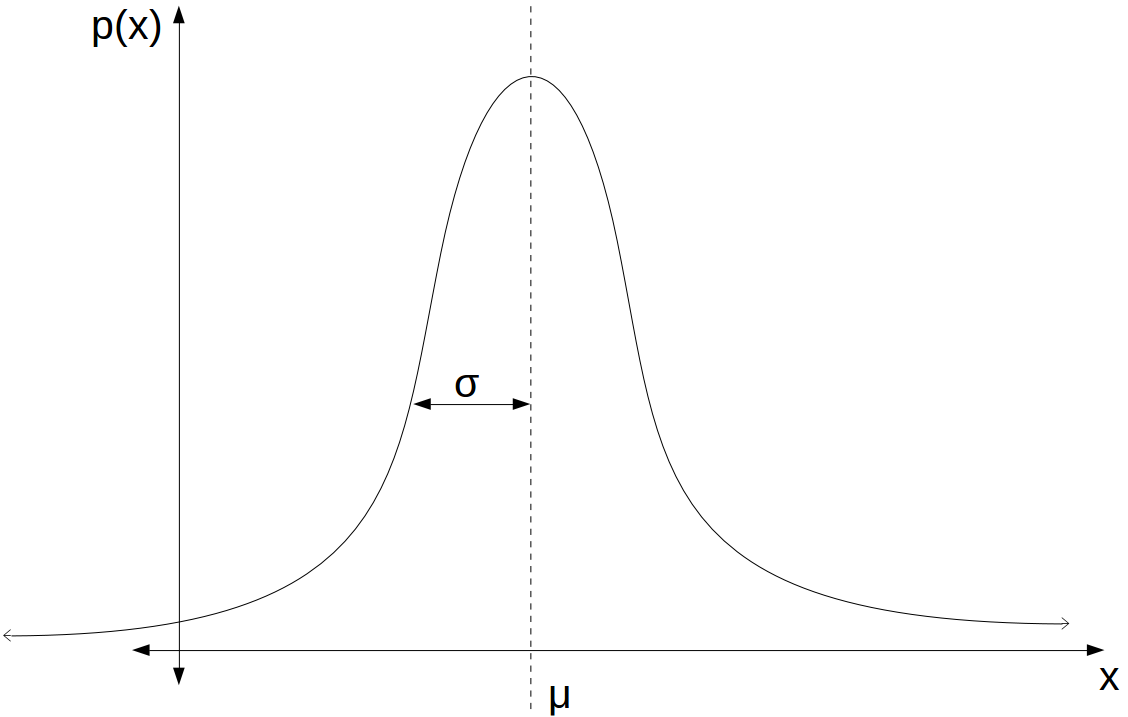
\includegraphics[width=0.6\linewidth]{Figures/univariate.png}
  \centering
  \caption{Univariate Gaussian PDF}
  \label{fig:gPDF1}
\end{figure}
The definition of the Gaussian distribution can be extended to describe the PDF of $N$ random variables (RVs). This is called the multivariate Gaussian distribution. The multivariate Gaussian distribution is described by an $N$-dimensional mean vector $\bm{\mu}$ and an $N\times N$ covariance matrix $\Sigma$. A random vector $\bm{x}$, with $N$ random variables (RVs), defined as
\begin{equation}
\bm{x} = [x_1\ ...\ x_N]^T,
\end{equation}
where $\bm{x}$ is drawn from a multivariate distribution which is described by a mean vector $\bm{\mu}$ and a covariance matrix $\Sigma$, defined as
\begin{equation}
\bm{x} \sim \mathcal{N}(\bm{x}; \bm{\mu},\Sigma).
\end{equation}
The PDF of $\bm{x}$ is defined as
\begin{equation}\label{eq:3}
p(\bm{x})  = \eta\exp\left[-\frac{1}{2}(\bm{x}-\bm{\mu})^T\Sigma^{-1}(\bm{x}-\bm{\mu})\right],
\end{equation}
where $\eta$ is a normalisation coefficient and is defined as
\begin{equation}\label{eq:4}
\eta = \frac{1}{(2\pi)^{\frac{N}{2}}|\Sigma|^{\frac{1}{2}}}.
\end{equation}

For this project it is required that $\Sigma$ is positive definite and thus also nonsingular, which guarantees a determinant that is nonzero. Positive definite covariance matrices are also invertible, thus the alternative canonical or information form, which requires $\Sigma^{-1}$, can be used. The canonical form is discussed in the following section.

The mean vector of RV vector $\bm{x}$ is equal to the expectation of $\bm{x}$ and is defined as
\begin{equation}
\bm{\mu} = E[\bm{x}].
\end{equation}
The covariance matrix $\Sigma$ specifies the correlation between RVs and is equal to
\begin{equation}\label{eq:defCovariance}
\begin{split}
\Sigma & = E\left[(\bm{x} - E[\bm{x}])^2\right]\\
& = E[\bm{xx}^T] - E[\bm{x}]E[\bm{x}]^T.
\end{split}
\end{equation}
\subsection{Error Ellipse}The following section is based on an article by Abdi ~\cite{abdi} and on a webpage from "Computer vision for dummies"~\cite{draw_ellipse}.

A multivariate Gaussian distribution with RV vector
\begin{equation}
\bm{x} = [x_1\ x_2]^T
\end{equation}
can be visualised as a series of ellipsoidal contours around the mean vector $\bm{\mu}$. The contours are an indication of the correlation between $x_1$ and $x_2$ and also show the uncertainty of the PDF. Contours close to one another suggest a steep incline and contours that are farther apart suggest a gradual incline in the PDF. Hence, small and concentrated contours represent certain Gaussian distributions and contours that are larger and farther apart represent uncertain Gaussian distributions. The drawing of error ellipses is an effective way to indicate the mean, the uncertainty and the correlation of a 2D Gaussian distribution.

An ellipse has a major axis and a minor axis as shown in Figure \ref{fig:e_ellipse}. The major axis of the error ellipse is always aligned in the direction in which the Gaussian distribution varies most. This direction can be found by determining the eigenvectors of the distribution. Each eigenvector has a corresponding eigenvalue which indicates the spread of the distribution in the direction of the eigenvector. 

We can use eigenvalue decomposition to factorise the covariance matrix $\Sigma$,
\begin{equation}
\Sigma = Q\Lambda Q^{-1}.
\end{equation}
Each column of the eigenvector matrix $Q$ contains an eigenvector $\bm{v}$. $Q$ is defined as
\begin{equation}
Q =
[\bm{v_1} \ \bm{v_2}]
=
\begin{bmatrix}
v_{11} & v_{21}\\
v_{12} & v_{22}
\end{bmatrix}.
\end{equation}
$\Lambda$ is a diagonal matrix and each of its diagonal entries contains an eigenvalue $\lambda$. $\Lambda$ is defined as 
\begin{equation}
\Lambda =
\begin{bmatrix}
\lambda_1 & 0\\
0 & \lambda_2
\end{bmatrix}.
\end{equation}
An error ellipse of a Gaussian PDF can be specified in terms of confidence levels, which is the probability that a value drawn from the distribution will fall inside the ellipse. Thus, differently sized ellipses can be plotted for different confidence levels. The lengths of the major an minor axes are sequentially specified as $2\sqrt{s\lambda_1}$ and $2\sqrt{s\lambda_2}$, where $\lambda_1 \geq \lambda_2$. The value of $s$ is determined by the confidence level of the error ellipse. In the case of an error ellipse with a confidence level of 95\%, $s$ is set to 5.991. The Chi-Square distribution can be used to find $s$ for other confidence levels, but it is beyond the scope of this document.

The orientation $\alpha$ of the error ellipse is shown in Figure \ref{fig:e_ellipse}. To obtain $\alpha$ we calculate the angle, relative to the x-axis, of the eigenvector with the largest spread. The angle $\alpha$ is defined as
\begin{equation}
\alpha = \arctan\left(\frac{v_{11}}{v_{12}}\right),
\end{equation}
where $\lambda_1 \geq \lambda_2$.

\begin{figure}[H]
  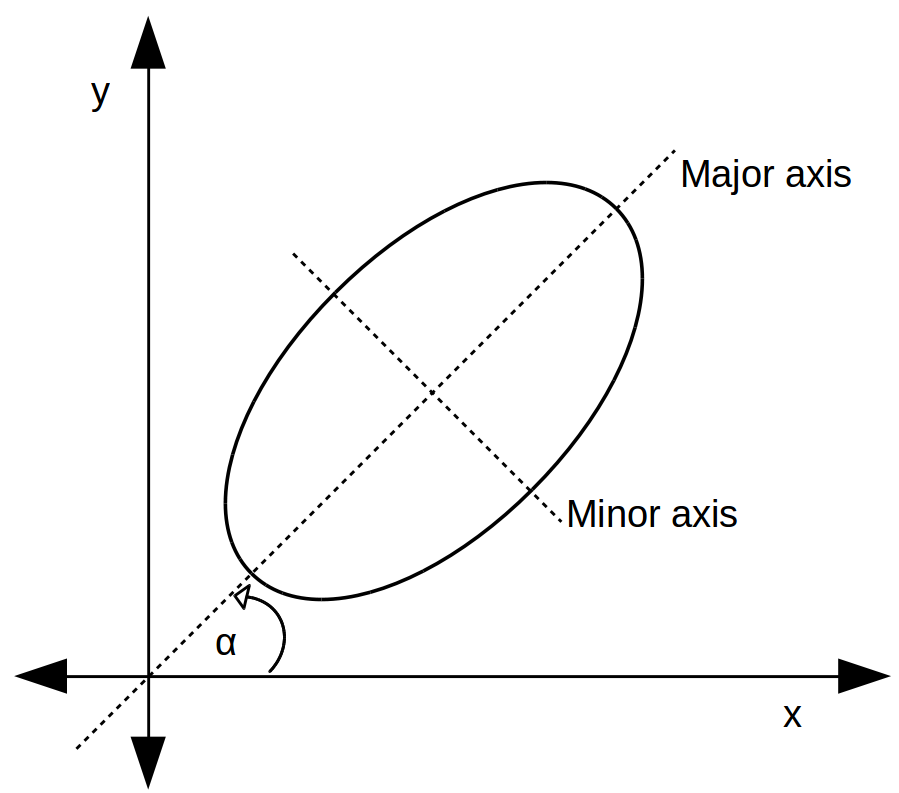
\includegraphics[width=0.5\linewidth]{Figures/e_ellipse.png}
  \centering
  \caption{Error Ellipse}
  \label{fig:e_ellipse}
\end{figure}
\section{Canonical Form}\label{sec:canonical}
The canonical or information form is an alternative way to describe Gaussian distributions. Using the canonical form has benefits, for example that certain operations are easier to perform. It can also be used to represent Gaussian conditional probability densities (CPDs), which will be discussed later in this section. This section is based on the work of Koller and Friedman~\cite{koller} and Schoeman~\citep{JC}.

The definition of the Gaussian distribution, shown in Equation \ref{eq:3}, can be rewritten in the following way
\begin{equation}
\begin{split}\label{eq:pdf_expand}
p(\bm{x}) & = \eta\exp\left[-\frac{1}{2}(\bm{x}-\bm{\mu})^T\Sigma^{-1}(\bm{x}-\bm{\mu})\right]\\
& = \exp\left(-\frac{1}{2}\bm{x}^T\Sigma^{-1}\bm{x} + \bm{\mu}^T\Sigma^{-1}\bm{x} - \frac{1}{2}\bm{\mu}^T\Sigma^{-1}\bm{\mu} + \ln{\eta}\right).
\end{split}
\end{equation}
We define the information matrix as
\begin{equation}\label{eq:defInfoMatrix}
K = \Sigma^{-1},
\end{equation}
the potential vector as
\begin{equation}\label{eq:defPotVec}
\bm{h} = \Sigma^{-1}\bm{\mu},
\end{equation}
and the scalar as
\begin{equation}\label{eq:defScalG}
g = - \frac{1}{2}\bm{\mu}^T\Sigma^{-1}\bm{\mu} + \ln{\eta}.
\end{equation}
We can substitute the definitions from Equation \ref{eq:defInfoMatrix} to Equation \ref{eq:defScalG} into Equation \ref{eq:pdf_expand}, and the define the canonical form as
\begin{equation}\label{eq:defCanonical}
\mathcal{C}(\bm{x}; K,\bm{h},g) = \exp\left(-\frac{1}{2}\bm{x}^TK\bm{x} + \bm{h}^T\bm{x} +g \right).
\end{equation}
Inspecting Equation \ref{eq:defInfoMatrix} to Equation \ref{eq:defScalG} again, it can be seen that one can always determine $g$, if the values of $\bm{h}$ and $K$ is available. The canonical form can thus be described in a simpler form as
\begin{equation}
\mathcal{C}(\bm{x}; K,\bm{h},g) \propto \mathcal{C}(\bm{x}; K,\bm{h}).
\end{equation}
One can easily recover the covariance parameters from the canonical parameters, where
\begin{equation}
\Sigma = K^{-1}
\end{equation}
and
\begin{equation}
\bm{\mu} = \Sigma\bm{h}.
\end{equation}
If $K$ is not invertible and the covariance can not be recovered, the canonical form is therefore more general than the covariance form.

It can be seen from the above that it is very easy to convert between the canonical and covariance forms. 
\subsection{Operations using the Canonical Form}
This section will cover useful operations using the canonical forms. 

Extending and rearranging the scopes of canonical forms may be necessary before doing operations, because it is important that the scopes of canonical forms are identical when doing operations. 
\subsubsection{Extending the Scope of a Canonical Form:}
The scope of a canonical form can be extended by adding zero entries to $K$ and $\bm{h}$. The scope of a canonical form of an $M$ sized random vector $\bm{x}$, can easily be extended to the size of $M + N$, by adding zeros in the following way:
\begin{equation}
\mathcal{C}\left(\bm{x};K,\bm{h}\right)
=
\mathcal{C}\left(
\begin{bmatrix}
\bm{x}\\
\bm{y}
\end{bmatrix};
\begin{bmatrix}
K & [0]_{M \times N}\\
[0]_{N \times M} & [0]_{N \times N}\\
\end{bmatrix},
\begin{bmatrix}
\bm{h}\\
\bm{0}
\end{bmatrix}
\right)
\end{equation}
\subsubsection{Rearranging the Scope of a Canonical Form:}
The scope can be rearranged by rearranging the rows and columns of $K$  and rearranging the entries of $\bm{h}$:
\begin{equation}
\mathcal{C}\left(
\begin{bmatrix}
\bm{x}\\
\bm{y}\\
\bm{z}
\end{bmatrix};
\begin{bmatrix}
K_{\bm{xx}} & K_{\bm{xy}} & K_{\bm{xz}}\\
K_{\bm{yx}} & K_{\bm{yy}} & K_{\bm{yz}}\\
K_{\bm{zx}} & K_{\bm{zy}} & K_{\bm{zz}}
\end{bmatrix},
\begin{bmatrix}
\bm{h_x}\\
\bm{h_y}\\
\bm{h_z}
\end{bmatrix}
\right)
=
\mathcal{C}\left(
\begin{bmatrix}
\bm{y}\\
\bm{x}\\
\bm{z}
\end{bmatrix};
\begin{bmatrix}
K_{\bm{yy}} & K_{\bm{yx}} & K_{\bm{yz}}\\
K_{\bm{xy}} & K_{\bm{xx}} & K_{\bm{xz}}\\
K_{\bm{zy}} & K_{\bm{zx}} & K_{\bm{zz}}
\end{bmatrix},
\begin{bmatrix}
\bm{h_y}\\
\bm{h_x}\\
\bm{h_z}
\end{bmatrix}
\right)
\end{equation}
\subsubsection{Multiplication of Canonical Forms:}
If the scopes of two canonical forms are identical, one can multiply them by simply adding the $K$ and $\bm{h}$ parameters of the two canonical forms:
\begin{equation}\label{eq:10}
\mathcal{C} (\bm{x}; K_{\bm{x}},\bm{h_x}) \times \mathcal{C} (\bm{y}; K_{\bm{y}},\bm{h_y})= \mathcal{C} (\bm{z};K_{\bm{x}} + K_{\bm{y}}, \bm{h_x} + \bm{h_y})
\end{equation}
%\subsubsection{Division of canonical forms:}
%Again, it important that the scopes of the distributions are identical.
%\begin{equation}\label{eq:11}
%\frac{\mathcal{C}(K_1,\bm{h_1},g_1)}{\mathcal{C}(K_2,\bm{h_2},g_2)} = %\mathcal{C}(K_1 - K_2,\bm{h_1} - \bm{h_2},g_1 - g_2)
%\end{equation}
\subsubsection{Marginalisation of a Canonical Form:}
A marginal distribution can be found by integrating over a subset of variables, for example the marginal distribution over $\bm{x}$ can be found by integrating over $\bm{y}$. Let $\mathcal{C}(\bm{x},\bm{y};K,\bm{h})$ be a canonical form with subsets $\bm{x}$ and $\bm{y}$ where
\begin{equation}
K = 
\begin{bmatrix}
K_{\bm{xx}} & K_{\bm{xy}}\\
K_{\bm{yx}} & K_{\bm{yy}}
\end{bmatrix}
\end{equation}
and
\begin{equation}
\ h = 
\begin{bmatrix}
h_{\bm{x}} \\
h_{\bm{y}}
\end{bmatrix}.
\end{equation}
To obtain the marginal distribution over $\bm{x}$, we have to find the integral over $\bm{y}$. Therefore the marginal distribution over $\bm{x}$ is
\begin{equation}
\int\mathcal{C}(\bm{x},\bm{y};K,\bm{h})d\bm{y} = \mathcal{C}(\bm{x};K',\bm{h}'),
\end{equation}
 where
\begin{equation}
K' = K_{\bm{xx}} - K_{\bm{xy}}K_{\bm{yy}}^{-1}K_{\bm{yx}}
\end{equation}
and
\begin{equation}
\bm{h'} = \bm{h}_{\bm{x}} - K_{\bm{xx}}K_{\bm{yy}}^{-1}\bm{h}_{\bm{y}}.
\end{equation}
It is important that $K_{\bm{yy}}$ is positive definite for the result to be finite.
\subsubsection{Reduction with Evidence:}
Let $\mathcal{C}(\bm{x},\bm{y};K,\bm{h})$ be a canonical form with subsets $\bm{x}$ and $\bm{y}$. If the value of subset $\bm{y}$ is known to be $\bm{Y}$, then the canonical form can be reduced to $\mathcal{C}(\bm{x}; K',\bm{h}')$, where
\begin{equation}
K' = K_{\bm{xx}},
\end{equation}
\begin{equation}
\bm{h'} = \bm{h}_{\bm{x}} - K_{\bm{xy}}\bm{Y},
\end{equation}

The operations discussed above are very simple to perform and will be used in the following chapters.
\subsection{Conditional Probability Distributions in the Canonical Form}
One of the advantages of the canonical form is that it is possible to represent conditional probability distributions (CPDs).

The CPD $p(\bm{y}|\bm{x})$ is a distribution of the vector $\bm{y}$, given we know the value of the vector $\bm{x}$, and is defined as
\begin{equation}
p(\bm{y}|\bm{x}) = \frac{p(\bm{y},\bm{x})}{p(\bm{x})}.
\end{equation}

If the arguments of the CPD $p(\bm{y}|\bm{x})$ can be described by a linear function
\begin{equation}
\bm{y} = F\bm{x} + \bm{g} + \bm{n},
\end{equation}
where
\begin{equation}
\bm{n} \sim \mathcal{N}(\bm{n}; \bm{0}, \Sigma_n),
\end{equation}
then the PDF of $p(\bm{y}|\bm{x})$ is defined as 
\begin{equation}
\label{eq:30}
\begin{split}
p(\bm{y}|\bm{x}) & = \mathcal{N}(\bm{y}; F\bm{x} + \bm{g}, \Sigma) \\
& = \eta\exp\left[-\frac{1}{2}(\bm{y} - (F\bm{x} + \bm{g}))^T\Sigma^{-1}(\bm{y}-(F\bm{x} + \bm{g}))\right].
\end{split}
\end{equation}
A part of Equation \ref{eq:30} can be rewritten as 
\begin{equation}\label{eq: rewrite}
\begin{split}
\bm{y} - (F\bm{x} + \bm{g}) & =
\begin{bmatrix}
I&-F&-I
\end{bmatrix}
\begin{bmatrix}
\bm{y}\\
\bm{x}\\
\bm{g}
\end{bmatrix}\\
& =
\begin{bmatrix}
I\\-F^T\\-I
\end{bmatrix}^T
\begin{bmatrix}
\bm{y}\\
\bm{x}\\
\bm{g}
\end{bmatrix}.
\end{split}
\end{equation}
Substituting Equation \ref{eq: rewrite} into Equation \ref{eq:30} gives
\begin{equation}
\label{eq:32}
\begin{split}
p(\bm{y}|\bm{x}) = \eta\exp\left[-\frac{1}{2}
\begin{bmatrix}
\bm{y}\\
\bm{x}\\
\bm{g}
\end{bmatrix}^T
\begin{bmatrix}
I\\-F^T\\-I
\end{bmatrix}
\Sigma^{-1}
\begin{bmatrix}
I\\-F^T\\-I
\end{bmatrix}^T
\begin{bmatrix}
\bm{y}\\
\bm{x}\\
\bm{g}
\end{bmatrix}
\right].
\end{split}
\end{equation}
We now define a new combined random vector
\begin{equation}\label{eq:ranVec}
\bm{w} = 
\begin{bmatrix}
\bm{y}\\
\bm{x}\\
\bm{g}

\end{bmatrix}
\end{equation}
and an information matrix
\begin{equation}\label{eq:newK}
K' =
\begin{bmatrix}
I\\-F^T\\-I
\end{bmatrix}
\Sigma^{-1}
\begin{bmatrix}
I\\-F^T\\-I
\end{bmatrix}^T.
\end{equation}
We can substitute Equation \ref{eq:ranVec} and Equation \ref{eq:newK} into Equation \ref{eq:32} which gives
\begin{equation}
\label{eq:35}
\begin{split}
p(\bm{y}|\bm{x}) = \eta\exp\left[-\frac{1}{2}
\bm{w}^T
K'
\bm{w}
\right].
\end{split}
\end{equation}
We can now use Equation \ref{eq:defCanonical} to write the conditional distribution of Equation \ref{eq:35} in the canonical form as follows
\begin{equation}\label{eq:linCan}
p(\bm{y}|\bm{x}) \propto \mathcal{C}(\bm{w}; K', \bm{0})\\
 =\mathcal{C}\left(
\begin{bmatrix}
\bm{y} \\
\bm{x} \\
\bm{g}
\end{bmatrix};
\begin{bmatrix}
I\\
-F^T\\
-I
\end{bmatrix}
\Sigma^{-1}
\begin{bmatrix}
I\\
-F^T\\
-I
\end{bmatrix}^T
, \bm{0}
\right)
\end{equation}
The parameter $\bm{g}$ is a constant and can be used as evidence to reduce the canonical form in Equation \ref{eq:linCan}, therefore
\begin{equation}\label{eq:conCanResult}
\begin{split}
\mathcal{C}(\bm{w}; K', \bm{0})& =\mathcal{C}\left(
\begin{bmatrix}
\bm{y} \\
\bm{x} \\
\end{bmatrix};
\begin{bmatrix}
I\\
-F^T
\end{bmatrix}
\Sigma^{-1}
\begin{bmatrix}
I\\
-F^T
\end{bmatrix}^T,
\begin{bmatrix}
I\\
-F^T
\end{bmatrix}
\Sigma^{-1}\bm{g}
\right)\\
& =\mathcal{C}\left(
\begin{bmatrix}
\bm{y} \\
\bm{x} \\
\end{bmatrix};
\begin{bmatrix}
\Sigma^{-1}  &  -\Sigma^{-1}F\\
-F^T\Sigma^{-1} & F^T\Sigma^{-1}F
\end{bmatrix}
, 
\begin{bmatrix}
-\Sigma^{-1}\bm{g}\\
-F^T\Sigma^{-1}\bm{g}
\end{bmatrix}
\right).
\end{split}
\end{equation}
This representation of conditional probability densities (CPDs) in the canonical form will be very useful in future chapters.
\chapter{Motion Models}\label{chap:motionModel}
Before locating a robot, it is important to model the way the robot moves. A simple linear motion model will be described which will later be used to illustrate basic principles when estimating the location of a linear moving robot. In practice the movement of a robot is seldom linear, therefore a more complex nonlinear motion model will also have to be explored. This chapter is based on the work of Thrun, Burgard and Fox~\citep{thrun}.
\section{Basic Concepts}
The motion model describes $p(\bm{x}_t|\bm{u}_t,\bm{x}_{t-1})$, which is the state transition probability density function (PDF). This is important and is used in the \textit{prediction step} of the Bayes filter, discussed in Chapter \ref{chap:kalmanFilter}. The material will cover kinematics in a stochastic form. Robot motion will be limited to planar movement to make it easier to convey concepts or ideas to the reader. Note that the theory discussed is not limited to planar movement and can easily be extended to three dimensions.

The kinematic state of a robot moving in a plane can be described by three variables which is referred to as the pose of the robot.
The pose is defined as
\begin{equation}
\bm{x_t} =
\begin{bmatrix}
x_t\\
y_t\\
\theta_t
\end{bmatrix}.
\end{equation}
As shown in Figure \ref{fig:pose_robot}, $x_t$ is the x-coordinate, $y_t$ is the y-coordinate and $\theta_t$ is the orientation of the robot at time $t$.

\begin{figure}[H]
  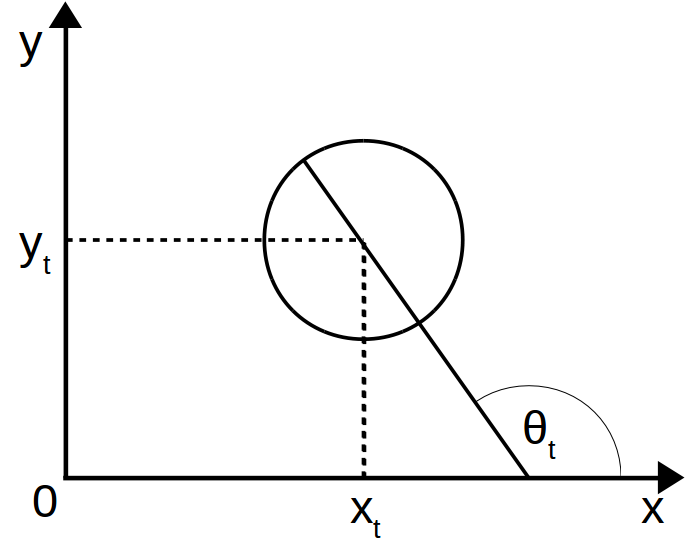
\includegraphics[width=0.4\linewidth]{Figures/pose_robot.png}
  \centering
  \caption{Robot pose}
  \label{fig:pose_robot}
\end{figure}
\section{Linear Motion Model}\label{sec:linearMotionModel}
This section describes the linear motion model. The parameter $\theta_t$ is omitted from the pose  and therefore the kinematic state of the robot is described only by a location
\begin{equation}
\bm{y_t} =
\begin{bmatrix}
x_t\\
y_t
\end{bmatrix}.
\end{equation}

The motion of the robot is independent of its orientation and can be controlled with two translational velocities in a control vector  $\bm{u}_t$, defined as
\begin{equation}
\bm{u_t} = 
\begin{bmatrix}
v_{x,t}\\
v_{y,t}
\end{bmatrix},
\end{equation}
where $v_{x,t}$ is the velocity in the x-direction and $v_{y,t}$ is the velocity in the y-direction at time $t$.

The position $\bm{y_t}$ of the robot at time $t$ can be described by a linear function in the form of
\begin{equation}\label{eq:lineartrans}
\bm{y_t} = A \bm{y_{t - 1}} + B \bm{u_t} + \bm{\varepsilon},
\end{equation}
where
\begin{equation}
A =
\begin{bmatrix}
1 & 0\\
0 & 1
\end{bmatrix},
\end{equation}
\begin{equation}
B = \begin{bmatrix}
\Delta t & 0\\
0 & \Delta t
\end{bmatrix},
\end{equation}
\begin{equation}
\bm{\varepsilon} =
\begin{bmatrix}
\varepsilon_x\\
\varepsilon_y
\end{bmatrix},
\end{equation}
and the noise is described as Gaussian distributions
\begin{equation}
\varepsilon_x \sim \mathcal{N}(\varepsilon_x; 0, \sigma_x^2),
\end{equation}
\begin{equation}
\varepsilon_y \sim \mathcal{N}(\varepsilon_y; 0, \sigma_y^2).
\end{equation}
The variances $\sigma_x^2$ and $\sigma_y^2$ are determined empirically and $\Delta t$ is the duration of a time interval.


\section{Nonlinear Motion Model}\label{vmodel}
Two nonlinear motion models were considered for this project, namely the velocity and odometry model. The odometry motion model makes use of sensor measurements to describe a robot's movement over time. Odometry models can  only be used in retrospect after a robot has moved and can not be used for motion planning. The velocity model is suitable for motion planning and assumes that a robot can be controlled with a rotational and translational velocity. The velocity motion model therefore predicts how the robot will move and is not as accurate as the odometry motion model. Both the odometry and velocity motion models are common and are widely used. As the velocity motion model meets the demands for the goal this project, it was chosen as the motion model.

The velocity motion model assumes that the movement of a robot can be described by a translational velocity $v_t$ and a rotational velocity $\omega_t$, shown in Figure \ref{fig:vel_model}. The control vector $u_t$ is thus described as
\begin{equation}
\bm{u_t} = 
\begin{bmatrix}
v_t\\
\omega_t
\end{bmatrix}.
\end{equation}
\begin{figure}
  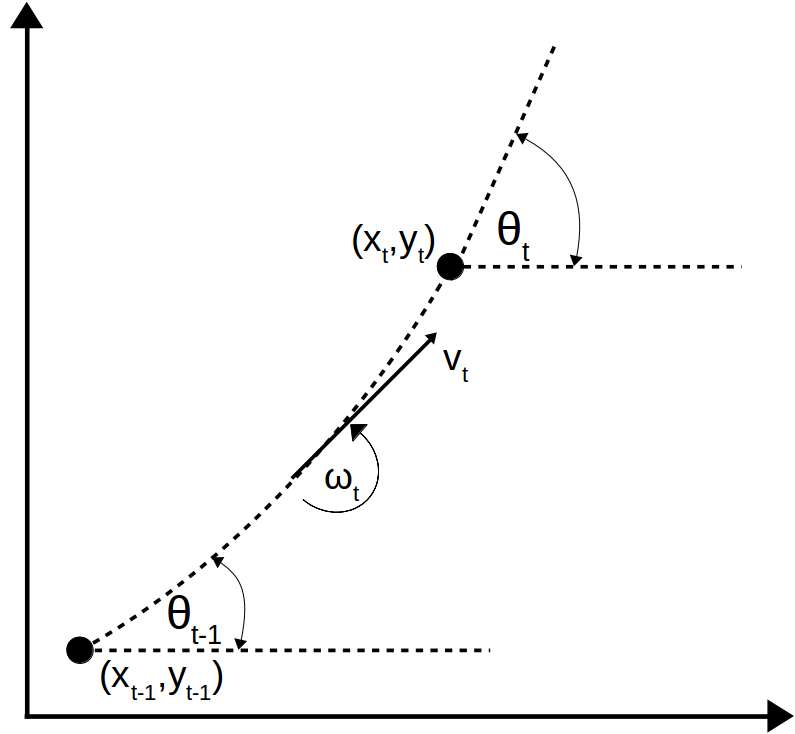
\includegraphics[width=0.4\linewidth]{Figures/velocity_model.png}
  \centering
  \caption{Velocity motion model}
  \label{fig:vel_model}
\end{figure}

Positive rotational velocities are defined to be counterclockwise and positive translational velocities are specified to be in the "forward" direction.
The pose at time $t$ can be determined by
\begin{equation}
\begin{bmatrix}
x_t\\
y_t\\
\theta_t
\end{bmatrix}
=
\begin{bmatrix}
x_{t-1} - \frac{v_t}{\omega_t} \sin\theta_{t-1} + \frac{v_t}{\omega_t} \sin(\theta_{t-1} + \omega_t \Delta t)\\
y_{t-1} + \frac{v_t}{\omega_t} \cos\theta_{t-1} - \frac{v_t}{\omega_t} \cos(\theta_{t-1} + \omega_t \Delta t)\\
\theta_{t-1} + \omega_t \Delta t
\end{bmatrix}+
\begin{bmatrix}
\varepsilon_x\\
\varepsilon_y\\
\varepsilon_\theta\\
\end{bmatrix},
\end{equation}
where
\begin{equation}
\varepsilon_x \sim \mathcal{N}(\varepsilon_x; 0, {\sigma_x}^2),
\end{equation}
\begin{equation}
\varepsilon_y \sim \mathcal{N}(\varepsilon_y; 0, {\sigma_y}^2)
\end{equation}
and
\begin{equation}
\varepsilon_\theta \sim \mathcal{N}(\varepsilon_\theta; 0, {\sigma_\theta}^2),
\end{equation}
and where variances ${\sigma_x}^2$, ${\sigma_y}^2$ and ${\sigma_\theta}^2$ are determined empirically.

The model is nonlinear due to the fact that the movement of the robot cannot be described by a linear translation in the form of
\begin{equation}
\bm{y} = A\bm{x} + B.
\end{equation}
%\chapter{Measurement Models}
%As mentioned in the introduction, measurements retrieved from %sensors always contain noise. A measurement model can be used% %one can describe it with a model. This chapter will describe %the linear measurement model and is based on Thrun~%%\citep{thrun}.
%\section{Linear Measurement Model}
\chapter{Localisation using Kalman Filters}\label{chap:kalmanFilter}
This chapter will focus on localisation using traditional techniques such as the Kalman filter, extended Kalman filter and unscented Kalman filter. This is important to investigate and understand as there is a strong correspondence to the PGM technique that will be discussed in a following section.
\section{Background}
A concept that is often used is in this report is that of \textit{belief}. As mentioned in the introduction, a robot cannot truly know its pose. A robot can infer a belief or have internal knowledge of its state from information gathered from sensors. There is thus a difference between internal belief and true state.

In this report the belief is a probability density function (PDF) of a state variable $\bm{x}_t$ given all the previous measurements $\bm{z}_{1:t}$  and controls $\bm{u}_{1:t}$ and is also known as the posterior. The belief of a state variable is denoted as
\begin{equation}
\bm{x}_t \sim bel(\bm{x}_t),
\end{equation}
which is a reduced notation for the posterior
\begin{equation}
bel(\bm{x}_t) = p(\bm{x}_t| \bm{z}_{1:t}, \bm{u}_{1:t}).
\end{equation}
The posterior $bel(\bm{x}_t)$ is usually calculated from a \textit{predicted belief} $\overline{bel}(\bm{x}_t)$, this calculation is known as the \textit{update step}.

The \textit{predicted belief} is defined as
\begin{equation}
\overline{bel}(\bm{x}_t) = p(\bm{x}_t|\bm{z}_{1:t-1}, \bm{u}_{1:t}),
\end{equation} 
and is the PDF of the state variable $\bm{x}_t$ without taking the measurement $\bm{z}_t$ in to consideration and it is known as the \textit{prediction step}.
\section{Bayes Filter}
The \textit{Bayes Filter} algorithm is the cornerstone for determining beliefs and filters such as the Kalman filter is a variation of it. The pseudo-algorithm for the Bayes filter is shown in Algorithm \ref{bayesAlg}. One can observe that the algorithm is recursive as it takes the previous belief $\bm{x}_{t-1}$ at time $t-1$ as an argument to estimate and return the belief $\bm{x}_t$ at time $t$. The algorithm takes three parameters, namely the previous belief $bel(\bm{x}_{t-1})$, the latest control input $\bm{u}_t$ and the measurements $\bm{z}_t$. The pseudo-algorithm shows one iteration of the algorithm that consists out of two steps, namely the \textit{prediction step} in line 3, and \textit{update step} in line 4.

The \textit{prediction step} calculates a predicted belief of the state $\bm{x}_t$ based on the previous state $\bm{x}_{t-1}$ and the control input $\bm{u}_t$. In this step the marginal distribution over $\bm{x}_{t-1}$ is calculated of the product of two distributions: the prior belief $bel(\bm{x}_{t-1})$, and the  transition probability $p(\bm{x}_t|\bm{u}_t,\bm{x}_{t-1})$.

In the \textit{update step} the final belief of state $\bm{x}_t$ is calculated by multiplying the predicted belief $\overline{bel}(\bm{x}_t)$ with the probability of $\bm{z}_t$ given $\bm{x}_t$. The result usually does not integrate to one, hence it is usually not a valid PDF and has to be normalized by multiplying it with $\eta$. The final belief $bel(\bm{x}_t)$ is returned.
\begin{algorithm}
\caption{Bayes Filter}\label{bayesAlg}
\begin{algorithmic}[1]
\Procedure{Bayes\_Filter}{$bel(\bm{x}_{t-1}), \bm{u}_t, \bm{z}_t$}
\ForAll{$\bm{x}_t$}
\State $\overline{bel}(\bm{x}_t) = \int p(\bm{x}_t|\bm{u}_t, \bm{x}_{t-1})bel(\bm{x}_{t-1})\, d\bm{x}_{t-1}$
\State $bel(\bm{x}_t) = \eta p(\bm{z}_t|\bm{x}_t) \overline{bel} (\bm{x}_t)$
\EndFor
\State \textbf{return} $bel(\bm{x}_t)$
\EndProcedure
\end{algorithmic}
\end{algorithm}

\section{Kalman Filter}
The Kalman filter is an implementation of the Bayes filter and is used for prediction in linear Gaussian systems. The Kalman filter is used for belief estimation of systems with continuous states and is not applicable in discrete state spaces. 
\subsection{Description of Kalman Filter}
The Kalman filter makes three assumptions in addition to the Markov assumptions which have the outcome that posterior beliefs calculated with the Kalman filter are Gaussian distributions.

1.Linear system dynamics are assumed. The motion model describing the movement must be linear with added Gaussian noise $\bm{\varepsilon}$ and must be able to express it with 
\begin{equation}\label{eq:linearKmm}
\bm{y}_t = A \bm{y}_{t - 1} + B \bm{u}_t + \bm{\varepsilon},
\end{equation}
with 
\begin{equation}
\bm{\varepsilon} \sim \mathcal{N}(\bm{\varepsilon}; \bm{0}, R_t)
\end{equation}
therefore the transition PDF $p(x_t|u_t, x_{t-1})$ is linear its arguments.

2. Linear measurements with Gaussian noise $\bm{\zeta}$ are assumed. The measurement PDF $p(z_t|x_t)$ is thus also linear in its arguments and can be described with
\begin{equation}
\bm{z}_t = C_t \bm{x}_t + \bm{\zeta}_t,
\end{equation} 
with
\begin{equation}
\bm{\zeta}_t \sim \mathcal{N}(\bm{\zeta}_t; \bm{0}, Q_t).
\end{equation}

3. The initial belief $bel(\bm{x}_0)$ of the system must be a Gaussian distribution.

The algorithm for the Kalman filter is shown in Algorithm \ref{kalAlg} and it is very similar to the Bayes filter in Algorithm \ref{bayesAlg}, as it is a variation of it. Line 1 and 2 of the Kalman filter is the \textit{prediction step} of the Bayes filter. The predicted mean $\overline{\bm{\mu}}_t$ and predicted covariance $\overline{\Sigma}_t $ is computed without including the measurements $z_t$ and describes the predicted belief $\overline{bel}(x_t)$. The previous mean $\bm{\mu}_t$ is transformed through the deterministic linear state transition function to determine the predicted mean $\overline{\bm{\mu}}$. The covariance $\Sigma_{t-1}$ is multiplied twice with $A_t$ and $R_t$ is added to determine the predicted covariance $\overline{\Sigma_t}$.

Line 4 to 6 corresponds with the \textit{update step} of the Bayes filter and the desired belief $bel(x_t)$ is computed and described by mean $\overline{\bm{\mu}}_t$ and covariance $\Sigma_t $. The Kalman gain $K_t$ is calculated in line 4 and is used to determine how much influence the measurements \bm{$z}_t$ has when it is incorporated. The difference between the actual measurements $\bm{z}_t$ and the expected measurements $C_t \bm{\overline{\mu}}_t$ is called the innovation. In line 5 the predicted mean $\overline{\bm{\mu}}_t$ is adjusted by summing it with the product of the Kalman gain and innovation. In line 6 the covariance $\Sigma_t$ is calculated. 
\begin{algorithm}
\caption{Kalman Filter}\label{alg:kalmanFilter}
\begin{algorithmic}[1]
\Procedure{Kalman\_Filter}{$\bm{\mu}_{t-1}, \Sigma_{t-1},\bm{u}_t, \bm{z}_t$}
\State $\overline{\bm{\mu}}_t = A_t \bm{\mu}_{t-1} + B \bm{u_}t$
\State $\overline{\Sigma}_t = A_t \Sigma_{t-1} A_t^T + R_t$
\State $K_t = \overline{\Sigma}_t C_t^T(C_t\overline{\Sigma}_t C_t^T + Q_t)^{-1}$
\State $\bm{\mu}_t = \overline{\bm{\mu}}_t + K_t(\bm{z}_t - C_t \overline{\bm{\mu}}_t)$
\State $\Sigma_t = (I - K_tC_t)\overline{\Sigma}_t$
\State \textbf{return} $\bm{\mu}_t, \Sigma_t$
\EndProcedure
\end{algorithmic}
\end{algorithm}

\subsection{Application of the Kalman Filter}
The Kalman filter was applied determine the belief of the location of a linear moving robot. The movement of the robot is described by the linear motion model in Section \ref{sec:linearMotionModel}. A moving robot was simulated in Python and the Kalman filter (Algorithm \ref{alg:kalmanFilter}) was implemented to find the belief $bel(\bm{x}_t)$ at each time step $t$.

The state transition function is defined as
\begin{equation}
\bm{y_t} = A \bm{y_{t - 1}} + B \bm{u_t} + \bm{\varepsilon},
\end{equation} 
where the matrix A is specified as
\begin{equation}
A =
\begin{bmatrix}
1 & 0\\
0 & 1
\end{bmatrix},
\end{equation}
the matrix B is specified
\begin{equation}
B =
\begin{bmatrix}
\Delta t & 0\\
0 & \Delta t
\end{bmatrix}, \Delta t = 1,
\end{equation}
and a Gaussian distribution describes the noise $\bm{\varepsilon}$ as
\begin{equation}
\bm{n} \sim \mathcal{N}(\bm{\varepsilon}; \bm{0}, R)
\end{equation}


\section{Extended Kalman Filter}
The Kalman filter discussed above is very efficient due to the fact that state transitions and measurements were assumed to be linear, hence them mean $\bm{\mu}_t$ and covariance $\Sigma_t$ of a resulting belief $bel(\bm{x}_t)$ can be computed analytically.
As mentioned in Chapter \ref{chap:motionModel}, state transitions and measurements are in reality rarely linear and therefore the normal Kalman filter is unsuitable for most robotics problems. In this project, only nonlinear state transitions were considered and measurements were assumed to be linear.

\subsection{Description of EKF}
The state transition of a nonlinear system can be described by
\begin{equation}
\bm{x}_t = \bm{g}(\bm{u}_t, \bm{x}_{t-1}) + \bm{\varepsilon}_t,
\end{equation}
and nonlinear measurements can be described by
\begin{equation}
\bm{z}_t = \bm{h}(\bm{x}_t) + \bm{\zeta}_t,
\end{equation}
where $\bm{h}$ and $\bm{g}$ are nonlinear vector functions. A Gaussian RV transformed through a nonlinear function results in a non-Gaussian RV, therefore the belief $bel(\bm{x}_t)$ is no longer Gaussian distributed and cannot be computed analytically.

The extended Kalman filter (EKF) is a variation on the Kalman filter and enables one to approximate a Gaussian distributed belief $bel({\bm{x}_t})$ of a system with nonlinear state transitions or measurements or both. The EKF linearises the functions $\bm{h}$ and $\bm{g}$ by means of Taylor expansion and as a result the belief $bel(\bm{x}_t)$ is approximated as a Gaussian distribution. 

In general, with Taylor expansion a nonlinear vector function
\begin{equation}\label{eq: taylorLin}
\bm{f}(\bm{x}) =
\begin{bmatrix}
f_1(\bm{x}) & ... & f_M(\bm{x})
\end{bmatrix}^T,
\end{equation}
with
\begin{equation}
\bm{x} =
\begin{bmatrix}
x_1 & ... & x_N
\end{bmatrix}^T,
\end{equation}
can be approximated as a linear vector function tangent to a given point $\bm{k}$ 
\begin{equation}
\bm{f}(\bm{x}) \approx \bm{f}(\bm{k}) + \bm{f}'(\bm{k})(\bm{x-k}),
\end{equation}
where the jacobian matrix
\begin{equation}\label{eq:jacobian}
\bm{f}'(\bm{x}) = \frac{\partial\bm{f}(\bm{x})}{\partial \bm{x}} =
\begin{bmatrix}
\frac{\partial f_1}{\partial x_1} & \dots &\frac{\partial f_1}{\partial x_N}\\
\vdots & \ddots &\vdots\\
\frac{\partial f_M}{\partial x_1} & \dots &\frac{\partial f_M}{\partial x_N}
\end{bmatrix}.
\end{equation}

Taylor expansion can be applied to linearise the nonlinear vector functions $\bm{g}$ and $\bm{h}$. Using  Equation \ref{eq: taylorLin}, $\bm{g}$ can be approximated as a linear vector function around $\bm{\mu}_{t-1}$
\begin{equation}\label{eq:linear_taylor}
\begin{split}
\bm{g}(\bm{u_t}, \bm{x}_{t-1}) & \approx \bm{g}(\bm{u}_t, \bm{\mu}_{t-1}) + \bm{g}'(\bm{u}_t, \bm{\mu}_{t-1})(\bm{x}_{t-1} - \bm{\mu}_{t-1})\\
& = \bm{g}(\bm{u}_t, \bm{\mu}_{t-1}) + G_t(\bm{x}_{t-1} - 
\bm{\mu}_{t-1}),
\end{split}  
\end{equation}
where $G_t$ is the jacobian matrix and can be determined by using Equation \ref{eq:jacobian}, therefore
\begin{equation}\label{eq:Gt}
G_t = \bm{g}'(\bm{u}_t, \bm{\mu}_{t-1}) = \frac{\partial \bm{g}(\bm{u}_t, \bm{x}_{t-1})}{\partial \bm{x}_{t-1}}.
\end{equation}
The same procedure can be followed to approximate the measurement function $\bm{h}$ as a linear vector function around the predicted mean $\overline{\bm{\mu}}$
\begin{equation}
\begin{split}
\bm{h}(\bm{x}_{t}) & \approx \bm{h}(\bm{\overline{\mu}}_{t}) + \bm{h}'(\bm{\overline{u}}_t)(\bm{x}_{t} - \bm{\overline{\mu}}_{t})\\
& = \bm{h}(\bm{\overline{\mu}}_t) + H_t(\bm{x}_{t} - 
\bm{\overline{\mu}}_{t}),
\end{split}  
\end{equation}
where
\begin{equation}\label{eq:Ht}
H_t = \bm{h}'(\bm{u}_t) = \frac{\partial \bm{h}(\bm{x}_{t})}{\partial \bm{x}_{t}}.
\end{equation}

In Algorithm \ref{EKFalg} the procedure of the EKF is shown and one will notice that is very similar to Algorithm \ref{alg:kalmanFilter} of the Kalman filter. The only difference is that the nonlinear state transition and measurement functions are linearised and therefore the state belief of the EKF is not exact.




\begin{algorithm}
\caption{Extended Kalman Filter}\label{EKFalg}
\begin{algorithmic}[1]
\Procedure{EKF}{$\bm{\mu}_{t-1}, \Sigma_{t-1},\bm{u}_t, \bm{z}_t$}
\State $\overline{\bm{\mu}}_t = \bm{g}(\bm{u}_t, \bm{\mu}_{t-1})$
\State $\overline{\Sigma}_t = G_t \Sigma_{t-1} G_t^T + R_t$
\State $K_t = \overline{\Sigma}_t H_t^T(H_t\overline{\Sigma}_t H_t^T + Q_t)^{-1}$
\State $\bm{\mu}_t = \overline{\bm{\mu}}_t + K_t(\bm{z}_t - h(\overline{\bm{\mu}}_t))$
\State $\Sigma_t = (I - K_tH_t)\overline{\Sigma}_t$
\State \textbf{return} $\bm{\mu}_t, \Sigma_t$
\EndProcedure
\end{algorithmic}
\end{algorithm}
This section covered the basic theory of the EKF, the next section will discuss how the EKF was implemented in Python.
\subsection{Application of EKF}
In this subsection the EKF is applied to localise a robot whose movement is described by the velocity motion model. Measurements of the robot's location were assumed to be linear. A moving robot with measurements were simulated and beliefs of the robot's pose were estimated using the EKF.

The robot's pose $\bm{x}_t$ at time $t$ is dependent on the previous pose $\bm{x}_{t-1}$ at time $t-1$ and the control $\bm{u}_t$. The transition of the robot's pose can be described in general as
\begin{equation}
\bm{x}_t =
\begin{bmatrix}
x_t\\
y_t\\
\theta_t
\end{bmatrix}
= \bm{g}(\bm{u}_t, \bm{x}_{t-1}) + \bm{\varepsilon},
\end{equation}
where the velocity motion model describes $\bm{g}$ as
\begin{equation}
\bm{g}(\bm{u}_t, \bm{x}_{t-1})=
\begin{bmatrix}
x_{t-1} - \frac{v_t}{\omega_t} \sin\theta_{t-1} + \frac{v_t}{\omega_t} \sin(\theta_{t-1} + \omega_t \Delta t)\\
y_{t-1} + \frac{v_t}{\omega_t} \cos\theta_{t-1} - \frac{v_t}{\omega_t} \cos(\theta_{t-1} + \omega_t \Delta t)\\
\theta_{t-1} + \omega_t \Delta t
\end{bmatrix}.
\end{equation}
The noise $\bm{\varepsilon}$ is defined as
\begin{equation}
\bm{\varepsilon} \sim \mathcal{N}(\bm{\varepsilon}; \bm{0}; R),
\end{equation}
where the covariance matrix R is defined as
\begin{equation}
R =
\begin{bmatrix}
\sigma_x^2 & 0 & 0\\
0 & \sigma_y^2 & 0\\
0 & 0 & \sigma_\theta^2
\end{bmatrix}.
\end{equation}
$R$ is a diagonal matrix, hence the noise added to each RV is independent.

The next step is to linearise the nonlinear vector function $\bm{g}$ by means of Taylor expansion. Equation \ref{eq:jacobian} and Equation \ref{eq:Gt} can be used to calculate the jacobian matrix $G_t$ of $\bm{g}$:
\begin{equation}\label{eq:velocityJacobian}
G_t = \bm{g}'(\bm{u}_t, \bm{x}_{t-1}) =
\begin{bmatrix}
1 & 0 & -\frac{v_t}{\omega_t} \cos\theta + \frac{v_t}{\omega_t} \cos(\theta + \omega_t \Delta t)\\
0 & 1 & -\frac{v_t}{\omega_t}\sin\theta + \frac{v_t}{\omega_t}\sin(\theta + \omega_t \Delta t)\\
0 & 0 & 1 
\end{bmatrix}.
\end{equation}
Using Equation \ref{eq:linear_taylor} and the jacobian matrix $G_t$ calculated in Equation \ref{eq:velocityJacobian}, the vector function $\bm{g}$ can be linearised around $\bm{u_{t-1}}$, thus
\begin{equation}\label{eq:linearG}
\bm{g}(\bm{u_t}, \bm{x}_{t-1}) \approx \bm{g}(\bm{u}_t, \bm{\mu}_{t-1}) + G_t(\bm{x}_{t-1} - 
\bm{\mu}_{t-1}).
\end{equation} 
Using the result in Equation \ref{eq:linearG}, the state transition in equation can be approximated as
\begin{equation}
\bm{x}_t \approx \bm{g}(\bm{u}_t, \bm{\mu}_{t-1}) + G_t(\bm{x}_{t-1} - \bm{\mu}_{t-1}) + \bm{\varepsilon}.
\end{equation} 
Linear measurements were assumed for the implementation and therefore
\begin{equation}
\bm{z}_t = C_t \bm{x}_t + \bm{\zeta}_t.
\end{equation}

For the simulation the robot was given ten different control inputs $\bm{u}_t$ and $\Delta t$ was set to one.
\section{Unscented Kalman Filter}\label{sec:UKF}
The linearisation used in the EKF is rudimentary, as nonlinear functions are linearised only around the mean which, in some scenarios, can lead to very inaccurate approximations. The unscented Kalman filter (UKF) is an alternative approach which in many cases deliver better results than that of the EKF, especially when $\bm{g}$ and $\bm{h}$ is highly nonlinear.

As mentioned before, a Gaussian distribution propagated through a nonlinear function results in a distribution that is non-Gaussian. The principle the UKF follows is to draw carefully chosen points called \textit{sigma points} around the mean from an existing Gaussian distribution and transform it through a nonlinear function. The transformed sigma points can then be used to approximate the resultant distribution as a Gaussian distribution.

Usually there is a sigma point located at the mean and two sigma points symmetrically around the mean for each dimension (along the main axes). For a $n$-dimensional Gaussian distribution there are $2n +1$ sigma points picked. Sigma points are denoted as
\begin{equation}
\mathcal{X}^{[i]},\ i\ = \ 1,\ ...,\ 2n,
\end{equation}
where $i$ indicates the index of the sigma point.

Sigma points are determined as follows:
\begin{flalign}
    &\mathcal{X}^{[0]} = \bm{\mu},& \\
    &\mathcal{X}^{[i]} = \bm{\mu} + \left(\sqrt{(n + \lambda)\Sigma}\right)\ \text{for}\ \ i =1, ...,n,&\\ 
    &\mathcal{X}^{[i]} = \bm{\mu} - \left(\sqrt{(n + \lambda)\Sigma}\right)\ \text{for}\ \ i = n + 1, ...,2n,&
\end{flalign}
where the scaling parameter $\lambda$ is defined as
\begin{equation}
\lambda = \alpha^2(n+\kappa) - n.
\end{equation}
The parameters $\alpha$ and $\kappa$ determines the spread of the sigma points around the mean.

Each sigma point $\mathcal{X}^{[i]}$ has corresponding weights $w_m^{[i]}$  and $w_c^{[i]}$, and is respectively used to recover the mean $\bm{\mu}_t$ and covariance $\Sigma_t$. Weights corresponding to $\mathcal{X}^{[0]}$, the mean $\bm{\mu}$ are determined as 
\begin{flalign}
    &w_m^{[0]} = \frac{\lambda}{n + \lambda},& \\ 
    &w_c^{[0]} = \frac{\lambda}{n+\lambda} + (1 - \alpha^2 + \beta).&
\end{flalign}
The parameter the optimal choice for the parameter $\beta$ is usually $2$.
The rest of the weights where $i = 1\ ,...,\ 2n$ are determined as
\begin{flalign}
    &w_m^{[i]} = w_c^{[i]} = \frac{1}{2(n + \lambda)}\ \ \text{for}\ i=1,\ ...,\ 2n.& 
\end{flalign}
After sigma points and weights have been calculated, the chosen sigma points can be transformed through a nonlinear vector function $\bm{f}$ to determine resulting sigma points $\mathcal{Y}^{[i]}$ and is given by 
\begin{equation}
\mathcal{Y}^{[i]} = \bm{f}\left(\mathcal{X}^{[i]}\right).
\end{equation}
The distribution as a result of the nonlinear transformation can be approximated as Gaussian distribution by estimating the mean $\bm{u}'$ and covariance $\Sigma'$ with 
\begin{equation}\label{eq:unscentedMean}
\bm{\mu}' = \sum_{i = 0}^{2n}w_m^{[i]}\mathcal{Y}^{[i]},
\end{equation}
\begin{equation}\label{eq:unscentedCov}
\Sigma' = \sum_{i=0}^{2n}w_c^{[i]}\left(\mathcal{Y}^{[i]} \right)
\end{equation}
The general theory of the UKF was covered in this section, the next section will discuss the implementation of the UKF.
\subsection{Application of UKF}
\begin{algorithm}
\caption{Unscented Kalman Filter}\label{UKFalg}
\begin{algorithmic}[1]
\Procedure{UKF}{$\bm{\mu}_{t-1}, \Sigma_{t-1},\bm{u}_t, \bm{z}_t$}
\State $\mathcal{X}_{t-1} = 
\begin{pmatrix}
\bm{\mu}_{t-1}  & \ \bm{\mu}_{t-1}+\gamma\sqrt{\Sigma_{t-1}} & \ \bm{\mu}_{t-1} - \gamma \sqrt{\Sigma_{t-1}})
\end{pmatrix}
$ 
\State $\overline{\mathcal{X}}^*_{t-1} = \bm{g}(\bm{u}_t, \mathcal{X}_{t-1})$
\State $\bm{\overline{\mu}}_t = \sum_i^{2n} w_m^{[i]} \overline{\mathcal{X}}^{*[i]}_{t}$
\State $\overline{\Sigma}_t = \sum_i^{2n}w_c^{[i]}\left(\mathcal{\overline{X}}_t^{*[i]} - \overline{\bm{\mu}}_t\right)\left(\mathcal{\overline{X}}_t^{*[i]} - \overline{\bm{\mu}}_t\right)^T +R_t$
\State $\mathcal{\overline{X}}_t = 
\begin{pmatrix}
\bm{\overline{\mu}}_{t}  & \ \bm{\overline{\mu}}_{t}+\gamma\sqrt{\overline{\Sigma_{t}}} & \ \bm{\overline{\mu}}_{t} - \gamma \sqrt{\overline{\Sigma_{t}}})
\end{pmatrix}$
\State $\overline{\mathcal{Z}}_t = \bm{h}\left(\mathcal{\overline{X}}_t\right)$
\State $\hat{\bm{z}}_t = \sum_{i=0}^{2n}w_m^{[i]} \overline{\mathcal{Z}}_t^{[i]}$ 
\State $S_t = \sum_{i=0}^{2n} w_c^{[i]}\left( \overline{\mathcal{Z}}_t^{[i]} - \hat{\bm{z}}_t  \right)\left( \overline{\mathcal{Z}}_t^{[i]} - \hat{\bm{z}}_t  \right)^T + Q_t$
\State $\overline{\Sigma}_t^{x,z} = \sum_{i=0}^{2n}  w_c^{[i]}\left( \overline{\mathcal{X}}_t^{[i]} - \overline{\bm{\mu}}_t  \right)\left( \overline{\mathcal{Z}}_t^{[i]} - \hat{\bm{z}}_t  \right)^T $
\State $K_t = \overline{\Sigma}_t^{x,z}S_t^{-1}$
\State $\bm{\mu}_t = \overline{\bm{\mu}}_t + K_t(\bm{z}_t - \hat{\bm{z}}_t)$
\State $\Sigma_t = \overline{\Sigma}_t - K_tS_tK_t^T$
\State \textbf{return} $\bm{\mu}_t, \Sigma_t$
\EndProcedure
\end{algorithmic}
\end{algorithm}

\chapter{Probabilistic Graphical Models}
This chapter gives a brief introduction to probabilistic graphical models which will later be used to solve the localisation problem with different techniques of numerical integration. PGMs are a very vast field, therefore only the theory relevant to this report will be covered. This chapter is based on the work of Koller and Friedman~\cite{koller}, Barber~\cite{barber} and Schoeman~\citep{JC}.
\section{Overview}
Reasoning about systems with uncertainty can become very complex and sometimes it is completely unmanageable. The PGM is a graphical technique which make problems tractable by modelling probabilistic systems in a logical and compact manner. PGMs are thus used to describe the relationship between variables and allows to reason about it. This action of querying a system or reasoning about a variable is called inference. It is a very popular technique, as it is intuitive, transparent and easy to manipulate. Hence, PGMs have countless applications from making medical diagnosis to localising robots.

PGMs used for modelling can be divided in to two categories. The first is Markov networks, which are used for non-causal systems. The second is Bayesian networks, where relationships between random variables are causal and specified as CPDs. As the localisation problem is in most cases causal, the focus of this chapter is on Bayesian networks.

Due to the relevance to localisation, the theory is discussed in terms of continuous random variables, but it can also be applied to discrete random variables. 
\section{Basic Concepts of Graphical Models}
There are a few basic concepts to understand before defining a Bayesian network. Graphical models consist of nodes and edges. Edges are the links between nodes and can be directed or undirected. Markov networks are undirected graphs, thus all edges are undirected. Bayesian networks are directed graphs, thus all edges are directed. An example of an undirected and directed graph can be seen in Figure \ref{fig:directed_graph} and Figure \ref{fig:undirected_graph} respectively.

In the case of directed graphs, nodes can be classified as ancestors, parents, children and descendants. If there exists a directed path from $x_1 \to x_k$, then $x_1$ is an ancestor of $x_k$, and $x_k$ is a descendant of $x_1$. In Figure \ref{fig:directed_graph}, $a$ is an ancestor of $c$ and $c$ is a descendant of $a$. A parent is an ancestor with only one edge between the ancestor and descendant. A child is a descendant with only one edge between the descendant and the ancestor. In Figure \ref{fig:undirected_graph}, $a$ is a parent of $b$ and $b$ is a child of $a$.~\cite{barber}

\begin{figure}[htbp]
  \begin{minipage}[b]{0.5\linewidth}
    \centering
    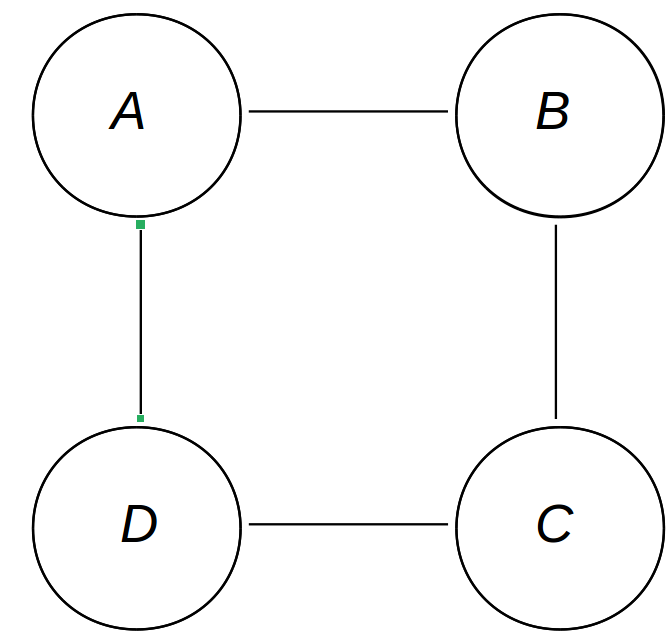
\includegraphics[width=0.5\linewidth]{Figures/undirected_graph.png}
    \caption{Directed graph}
    \label{fig:directed_graph}
  \end{minipage}
  \hspace{0.5cm}
  \begin{minipage}[b]{0.5\linewidth}
    \centering
    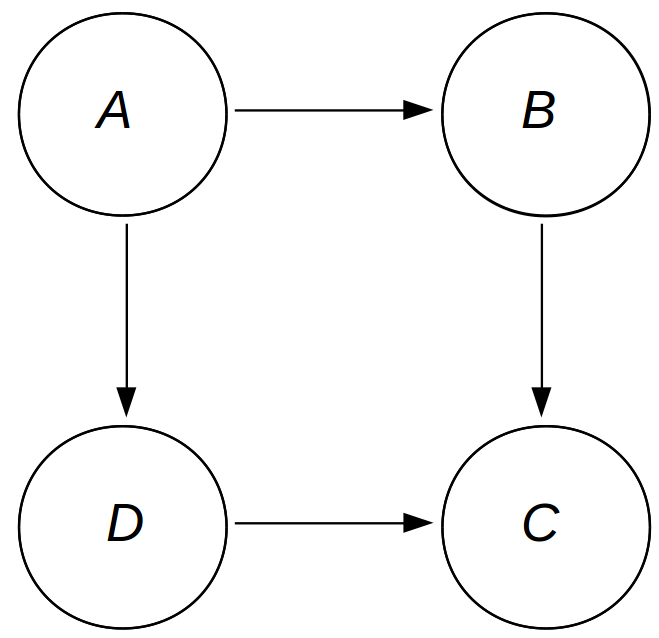
\includegraphics[width=0.5\linewidth]{Figures/directed_graph.png}
    \caption{Undirected graph}
    \label{fig:undirected_graph}
  \end{minipage}
\end{figure}

\section{Bayesian Networks}
Bayesian networks consists of random variables in the form of nodes and are connected by directed edges. Nodes that are not directly connected to each other, are considered conditionally independent. Relationships between nodes are indicated as conditional probability distributions (CPDs) and each node can be associated with a CPD
\begin{equation}
x_i \sim p(x_i|Par(x_i)),
\end{equation}
where $Par(x_i)$ indicates the parents of node $x_i$.

CPDs can be written as a factors. A factor is a function that takes a number of random variables as arguments and is defined as
\begin{equation}
\phi_i(x_i, Par(x_i)) = p(x_i|Par(x_i)),
\end{equation}
where the scope of a factor is its arguments 
\begin{equation}
\text{Scope}\{\phi_i\} = \{x_i, Par(x_i)\}.
\end{equation}
The concept of a factor is important that will be used in the rest of the report.

Figure \ref{fig:bays_pgm} shows an example of a Bayesian network with seven nodes labelled from $a$ to $g$. Each node is associated with a CPD. Directed edges between nodes are indicated with arrows.
\begin{figure}[H]
  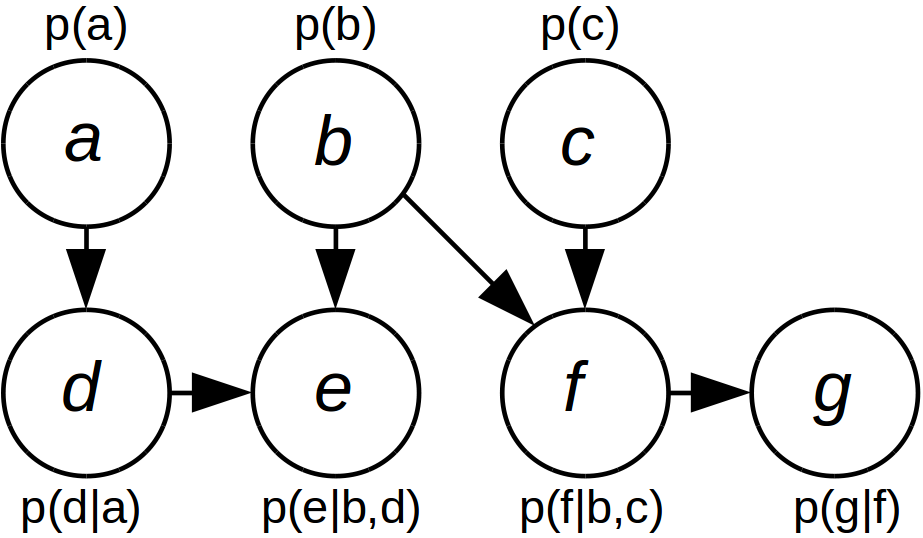
\includegraphics[width=0.5\linewidth]{Figures/bayesian_pgm.png}
  \centering
  \caption{Bayesian network}
  \label{fig:bays_pgm}
\end{figure}
The chain rule specifies that the joint probability density distribution of all the variables in a Bayesian network can be found by finding the product of all the CPDs associated with nodes~\citep{koller} and is defined as
\begin{equation}
p(x_1, ..., x_n) = \prod_i p(x_i|Par(x_i)).
\end{equation}
The chain rule can be applied to the Bayesian network in Figure \ref{fig:bays_pgm}
\begin{equation}
p(a,b,c,d,e,f,g) = p(a)p(b)p(c)p(d|a)p(e|b,d)p(f|b,c)p(g|f)
\end{equation}
A marginal PDF of the subset of variables $a$, $b$ and $c$ can be found by integrating over all the variables not in the subset, therefore
\begin{equation}
p(a,b,c) = \int\int\int\int p(a,b,c,d,e,f,g)dd\,de\,df\,dg.
\end{equation}
The chain rule together with marginalisation can be used to inference a Bayesian network, but it can be very tedious. The next section covers an alternative method to inference Bayesian networks in a structured manner.
\section{Cluster Graphs}
The next step is to reason about variables of a Bayesian network in a more efficient manner. Various methods can be used to inference a Bayesian network; one method is to construct a cluster graph. The cluster graph consists of clusters connected by undirected edges.

Clusters can be formed by grouping factors together such that each cluster $C_i$ is subset of the variables of the Bayesian network
\begin{equation}
C_i \subseteq \{x_1, ..., x_n\}.
\end{equation}
The undirected edges between clusters are called sepsets and are responsible for passing messages between clusters. A sepset between two clusters contains information about variables that are common to both clusters. An edge between $C_i$ and cluster $C_j$ is associated with a sepset with a subset of variables that is common to both $C_i$ and $C_j$ and is defined as
\begin{equation}
S_{i,j} \subseteq C_i \cap C_j.
\end{equation}
There are multiple ways to construct clusters, but it should adhere to two requirements~\citep{koller}:

1. Family preservation requires that every factor $\phi_k$ in a Bayesian network with a set of factors $\Phi$, there exists a cluster $C_i$ which accommodates $\phi_k$
\begin{equation}
\text{Scope}[{\phi}_k] \subseteq C_i.
\end{equation}

2. The running intersection property states that there exists an unique path connecting a pair of clusters containing the same variable $x$, and every cluster and sepset along the path also contain $x$. This path allows clusters to share their beliefs of $x$. In other words, for any variable $x$, the set of sepsets and clusters containing $x$ form a tree~\citep{koller}. This prevents feedback loops and thus counters the phenomena where clusters reinforce their own beliefs of variables.

Figure \ref{fig:bays_pgm} is converted in Figure \ref{fig:cluster_bound} where CPDs are replaced with factors and possible cluster boundaries are indicated with dashed rectangles. Note that there are other ways to construct the cluster graph.
\begin{figure}[H]
  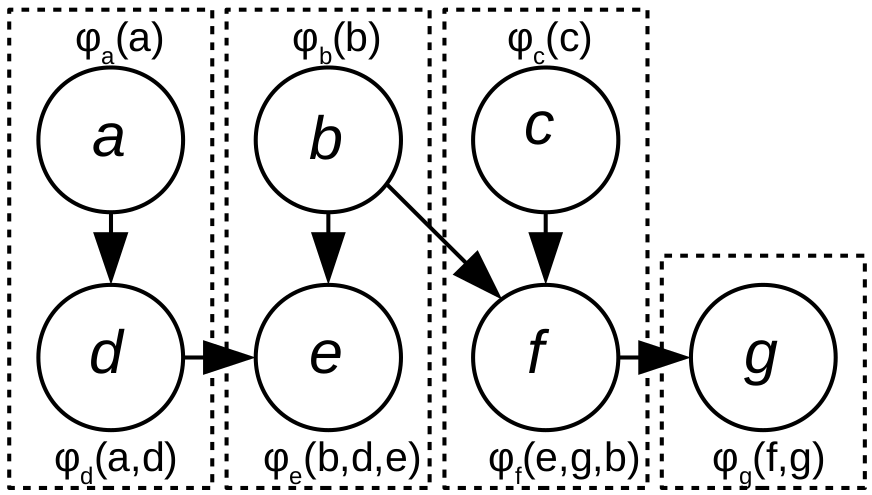
\includegraphics[width=0.6\linewidth]{Figures/cluster_divisions.png}
  \centering
  \caption{Bayesian network with cluster boundaries}
  \label{fig:cluster_bound}
\end{figure}

The initial belief of a cluster can be calculated by finding the product of all the factors inside the cluster~\citep{koller}. The initial belief of a cluster is defined as
\begin{equation}
\psi_i(C_i) = \prod_{k}\phi_k.
\end{equation}
Figure \ref{fig:cluster_bound} is transformed in Figure \ref{fig:clustergraph}. Clusters are indicated by ellipsis. Initial beliefs are calculated and shown inside the ellipsis. Sepsets are indicated by rectangles.
\begin{figure}[H]
  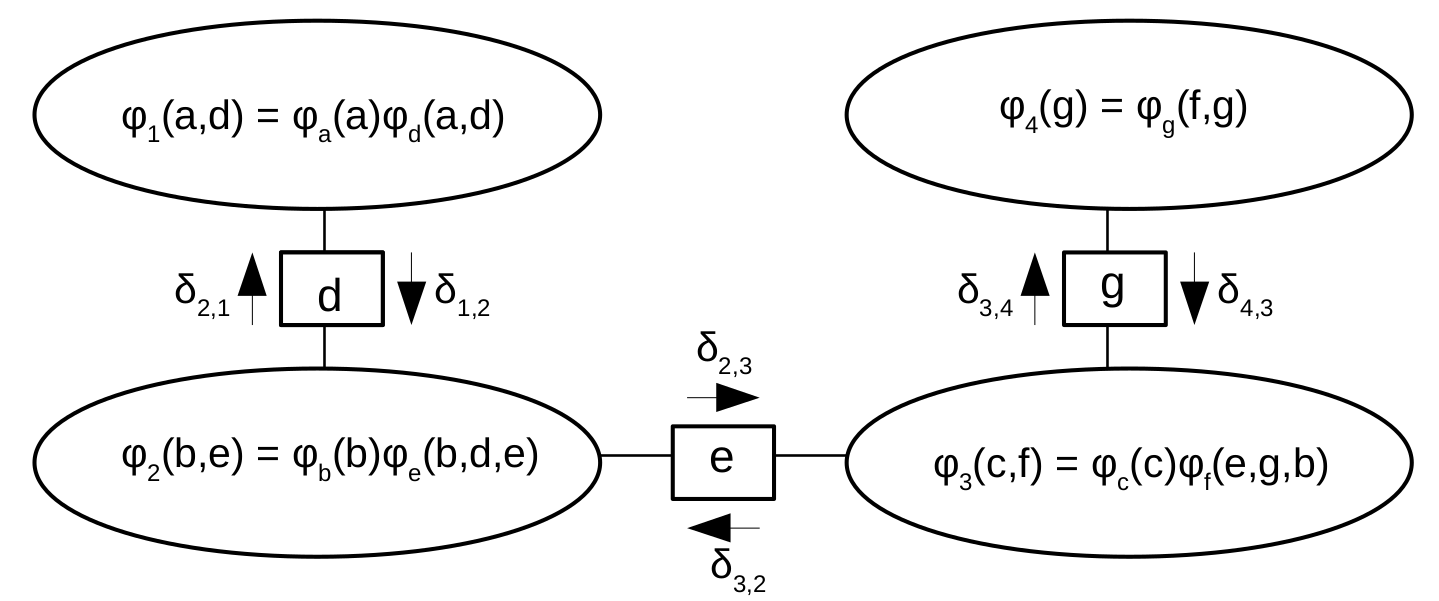
\includegraphics[width=0.7\linewidth]{Figures/clustergraph.png}
  \centering
  \caption{Cluster graph showing sepsets and clusters with initial beliefs}
  \label{fig:clustergraph}
\end{figure}
This section showed how to construct a cluster graph with clusters and sepsets. The cluster graph allows clusters to share beliefs of variables by means of message passing which will be explored in the next section. 
\section{Message Passing}
Clusters can share beliefs of common variables using message passing. Every sepset $S_{i,j}$ has two messages, $\delta_{i, j}$ and $\delta_{j,i}$, associated with it. This allows clusters, connected by a sepset, to communicate in both directions. An outgoing message $\delta_{i,j}$ of a cluster $C_i$ can be calculated by multiplying the initial cluster belief $\psi_i$ with all the incoming messages $\delta_{k,j}$ from other clusters $C_k$ and then marginalising onto the variables contained in the sepset $S_{i,j}$, thus integrating over variables not in the sepset ie. $C_i - S_{i,j}$. This procedure is defined as~\citep{koller}
\begin{equation}\label{eq:messageOut}
\delta_{i,j}(S_{i,j}) = \int_{C_i - S_{i,j}}\psi_i \times \prod_{k\ne j} \delta_{k,i}(S_{k,i}).
\end{equation}
Equation \ref{eq:messageOut} can be demonstrated by calculating arbitrary messages $\delta_{2,3}$ and in $\delta_{3,4}$ Figure \ref{fig:clustergraph}, therefore
\begin{equation}
\delta_{2,3}(b) = \int_d \int_e \delta_{1,2}(d)\psi_2(b,d,e)dd\ de
\end{equation}
and
\begin{equation}
\delta_{3,4}(f) = \int_b \int_c \delta_{2,3}(b)\psi_3(b,c,f)db\ dc.
\end{equation}

Sometimes the value of a RV in a PGM is known, in other words there is evidence of a RV available. Evidence of random variables is available to the entire PGM, therefore after evidence of a RV is inserted the RV itself doesn't appear in the PGM any more. Evidence is indicated by a capital letter, thus $X$ is evidence of the RV $x$. Evidence is used to reduce a PDF before calculating messages.

In Equation \ref{eq:evidence}, an outgoing message $\delta_{i , j}(y)$ is calculated. Evidence of $x$ is available and is indicated as $X$. The evidence of $x$ is used to reduce the cluster $\psi_i$ before multiplying it with all incoming messages and integrating over $z$.
\begin{equation}\label{eq:evidence}
\delta_{i , j}(y) = \int_{z}\psi_i(x = X, y, z) \times \prod_{k\ne j} \delta_{k , i}(S_{k,i})
\end{equation}
After all the incoming messages of a cluster have been determined, the belief of a cluster can be calculated by multiplying the cluster's initial belief with all of the incoming messages, and normalising the end result. Koller and Friedman~\cite{koller} specifies this as
\begin{equation}
\beta_i(C_i) \propto \psi_i \times \prod_{k} \delta_{k , i}(S_{k,i}).
\end{equation}

This chapter covered the properties of the Bayesian network and how one can reason about a Bayesian network by constructing a cluster graph. The Bayesian network will be used in the next chapter to model the localisation problem.
\chapter{Localisation using Probabilistic Graphical Models}
In this chapter a PGM will be used as an alternative method to reason about a causal localisation problem. The problem is modelled with a Bayesian network in Section \ref{sec:model} and in Section \ref{sec:cluster} a cluster graph is constructed to reason about the location of the robot. This technique then is compared to that of the Bayes filter in Algortim \ref{bayesAlg} and it is investigated where numerical integration is needed when reasoning about a RV in a nonlinear system.

\section{Modelling the Localisation problem}\label{sec:model}
A Bayesian network is used to model the localisation problem and is shown in Figure \ref{fig:loc_bayes}. There are nodes representing the control $\bm{u}_t$, the state of the robot $\bm{x}_t$ and the measurement $\bm{z}_t$ at each time step ($t = 1,\ ..,T$). The relationship between nodes are indicated as conditional probability densities (CPDs) and can also be written as factors, where
\begin{equation}
\phi_{\bm{u}_t}(\bm{u}_t) = p(\bm{u}_t),
\end{equation}
\begin{equation}
\phi_{\bm{x}_t}(\bm{x}_t, \bm{u}_t, \bm{x}_{t-1}) = p(\bm{x}_t| \bm{u}_t, \bm{x}_{t-1}) 
\end{equation}
and
\begin{equation}
\phi_{\bm{z}_t}(\bm{z}_t, \bm{x}_t) = p(\bm{z}_t|\bm{x}_t). 
\end{equation}
The current state of the robot's pose $\bm{x}_t$ is dependent on the previous state $\bm{x}_{t-1}$ and control $\bm{u}_t$. The measurement $\bm{z}_t$ is dependent on the state $\bm{x}_t$. The belief of the initial state $bel(\bm{x}_0)$ is known, and the values of the control vectors $\bm{u}_t$ and measurement vectors $\bm{z}_t$ are given as evidence by $\bm{U}_t$ and $\bm{Z}_t$, respectively.

\begin{figure}
  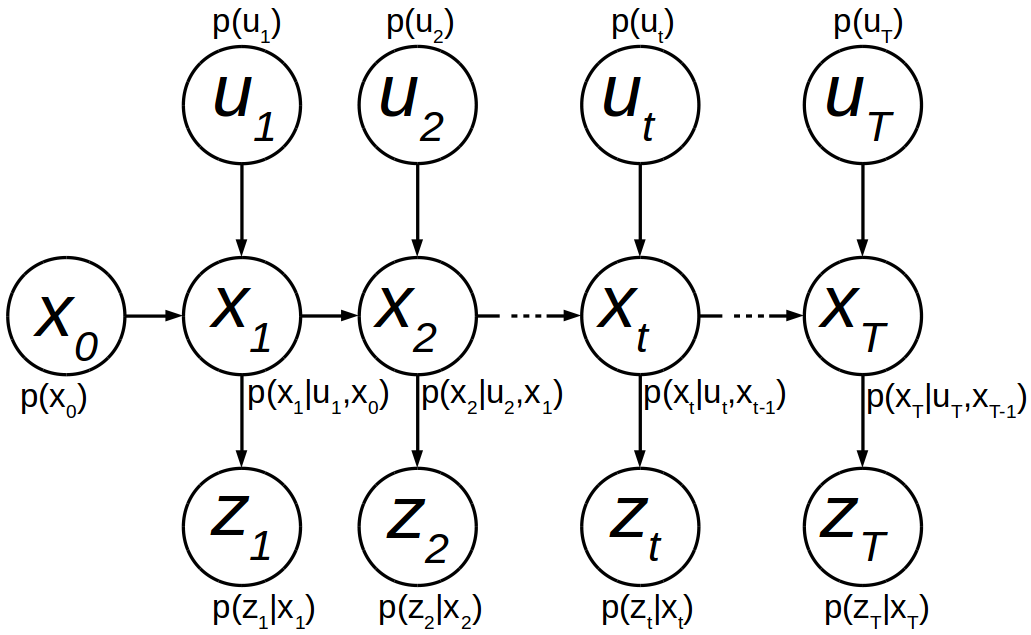
\includegraphics[width=0.7\linewidth]{Figures/bayesnetloc.png}
  \centering
  \caption{Bayesian network of localisation problem}
  \label{fig:loc_bayes}
\end{figure}
\section{Reasoning with a Cluster Graph}\label{sec:cluster}
The Bayesian network in Figure \ref{fig:loc_bayes} is converted to a cluster graph, shown in Figure \ref{fig:loc_cluster}. The cluster graph allows one to reason about the RVs of the Bayesian network. There are a numerous ways to group the factors to form clusters. In this cluster graph factors $\phi_{\bm{u}_t}, \phi_{\bm{x}_t}$ and $\phi_{\bm{z}_t}$  at each time step $t$  were grouped together to form a cluster $C_t$. The cluster factor of each cluster $C_t$ can be determined as
\begin{equation}
\psi_t(\bm{x}_t, \bm{x}_{t-1}, \bm{u}_t, \bm{z}_t) = \phi_{\bm{x}_t}(\bm{x}_t,\bm{u}_t,\bm{x}_{t-1})\phi_{\bm{z}_t}(\bm{z}_t,\bm{x}_t)\phi_{\bm{u}_t}(\bm{u}_t).
\end{equation}

\begin{figure}
  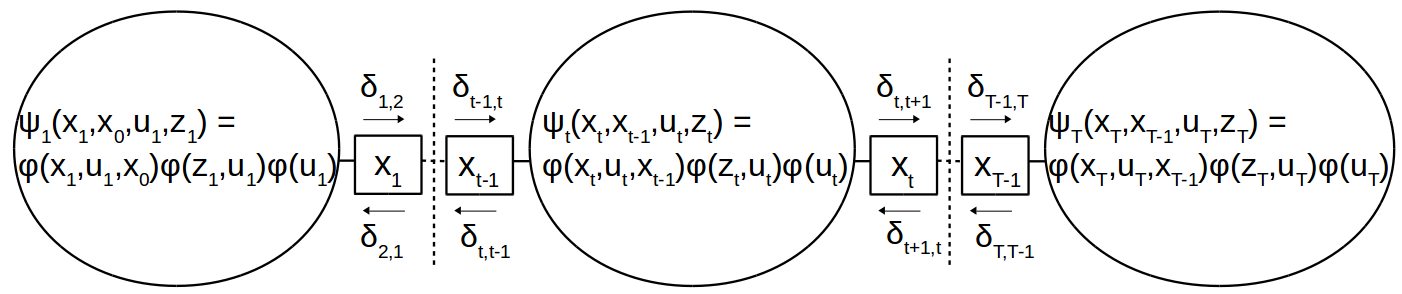
\includegraphics[width=\linewidth]{Figures/loc_clustergraph.png}
  \centering
  \caption{Cluster graph with grouped factors and sepsets}
  \label{fig:loc_cluster}
\end{figure}

Sepsets between clusters are indicated with rectangles and allows clusters to reason about mutual variables by means of message passing. In Figure \ref{fig:loc_cluster} messages associated with sepsets are shown in both directions, but for this causal example only messages in the "forward" direction were calculated. The messages pointing from right to left can also be determined and then used to sent information "backwards" in time which can lead to better estimates of beliefs at previous time steps. The process where messages are sent in both directions are known as smoothing.

The initial belief $bel(\bm{x}_0)$ is known and can be viewed as the only incoming message of cluster $C_1$. One can therefore calculate the messages of the cluster graph in Figure \ref{fig:loc_cluster} by starting at the very left cluster, $C_1$, and then calculate each cluster's outgoing message, in a consecutive order.
Applying Equation \ref{eq:messageOut} to calculate an general outgoing message $\delta_{t,t+1}(\bm{x}_t)$ of a cluster $C_t$, one can observe that
\begin{equation}\label{eq:mesBel}
bel(\bm{x}_t) = \eta\delta_{t,t+1}(\bm{x}_t).
\end{equation}
The observation in Equation \ref{eq:mesBel} and Equation \ref{eq:messageOut} can be used to calculate a belief $bel(\bm{x}_t)$, therefore
\begin{equation}\label{eq:outMes}
\begin{split}
bel(\bm{x}_t) & = \eta \delta_{t,t+1}(\bm{x}_t)\\
& = \eta \int_{\bm{x}_{t-1}}\phi_{\bm{x}_t}(\bm{x}_t,\bm{u}_t,\bm{x}_{t-1})\phi_{\bm{z}_t}(\bm{z}_t,\bm{x}_t)\phi_{\bm{u}_t}(\bm{u}_t)\delta_{t-1,t}(\bm{x}_{t-1})\,d\bm{x}_{t-1}\\
& = \eta \int_{\bm{x}_{t-1}}\phi_{\bm{x}_t}(\bm{x}_t,\bm{u}_t,\bm{x}_{t-1})\phi_{\bm{z}_t}(\bm{z}_t,\bm{x}_t)\phi_{\bm{u}_t}(\bm{u}_t =\bm{U}_t)bel(\bm{x}_{t-1})\,d\bm{x}_{t-1}\\
& = \eta \phi_{\bm{z}_t}(\bm{z}_t,\bm{x}_t)\int_{\bm{x}_{t-1}}\phi_{\bm{x}_t}(\bm{x}_t,\bm{u}_t,\bm{x}_{t-1})bel(\bm{x}_{t-1})\,d\bm{x}_{t-1}.
\end{split}.
\end{equation}
The result of Equation \ref{eq:outMes} can be written in terms of CPDs, therefore
\begin{equation}\label{eq:pgmBayesEq}
bel(\bm{x}_t) = \eta p(\bm{z}_t|\bm{x}_t)\int_{\bm{x}_{t-1}}p(\bm{x}_t|\bm{u}_t,\bm{x}_{t-1})bel(\bm{x}_{t-1})\,d\bm{x}_{t-1}.
\end{equation}
Equation \ref{eq:pgmBayesEq} can be compared to Algorithm \ref{bayesAlg} and can be seen that the procedure of operations is identical to that of the Bayes filter, this shows that reasoning about the state of a robot in a causal system by means of a PGM will give the same result as when the Bayes filter is used. The method of using the PGM is a very general way to represent the problem and can be considered superior to the Bayes filter, as the PGM can be easily changed by adding or removing nodes. PGMs can also be used to model various systems and is not restricted to the localisation problem.

\section{Numerical Integration}
The previous section uses a PGM to reason about thg belief $bel(\bm{x}_t)$ in a generic way. This is useful as different methods can easily be implemented to do operations of Equation \ref{eq:outMes}. In this project the canonical form was used to represent and to do operations on factors. If all the factors of Equation \ref{eq:outMes} can be represented with the canonical form, the result can easily be computed. However, a conditional probability distribution (CPD) that is described by a nonlinear function is usually not a Gaussian distribution and cannot be represented with the canonical form. This section investigates three methods to approximate nonlinear transformations of CPDs as linear transformations which will enable one to approximate the belief in Equation \ref{eq:outMes} as a Gaussian distribution.

\subsection{Taylor Series Expansion}
The first method uses Taylor series expansion to a linearise nonlinear functions associated with CPDs. This is not numerical integration as the functions are linearised and the Jacobian matrix of each function must be determined beforehand.
Equation \ref{eq: taylorLin} to Equation \ref{eq:Ht} is used to linearise the state transition function $\bm{h}$ and measurement function $\bm{g}$.
The linearised functions can be represented by the canonical form by implementing it in the the result of Equation \ref{eq:linCan}. The state transition function
\begin{equation}\label{eq:nonLinStateTransFunc}
\bm{x}_t = \bm{g}(\bm{u}_t, \bm{x}_{t-1}) + \bm{\varepsilon}_t,
\end{equation}
where
\begin{equation}
\bm{\varepsilon}_t \sim \mathcal{N}(\bm{\varepsilon}, \bm{0}, R_t).
\end{equation}
The nonlinear function, $\bm{g}$, in Equation \ref{eq:nonLinStateTransFunc} can be linearised by means of Taylor expansion. The state transition in Equation \ref{eq:nonLinStateTransFunc} can now be approximated as
\begin{equation}\label{eq:taylorCanLin1}
\bm{x}_t \approx \bm{g}(\bm{u}_t, \bm{\mu}_{t-1}) + G_t(\bm{x}_{t-1} - 
\bm{\mu}_{t-1}) + \bm{\varepsilon}_t.
\end{equation}
The result of Equation \ref{eq:taylorCanLin1} can be written in the form $\bm{y} = F\bm{x} + \bm{g} + \bm{n}$:
\begin{equation}\label{eq:taylorCanLin2}
\bm{x}_t \approx G_t\bm{x}_{t-1} + (\bm{g}(\bm{u}_t, \bm{\mu}_{t-1}) - G_t\bm{u}_{t-1}) + \bm{\varepsilon}_t.
\end{equation}

By implementing the result of Equation \ref{eq:taylorCanLin2} in Equation \ref{eq:conCanResult}, the state transition distribution $p(\bm{x}_t|\bm{u}_t,\bm{x}_{t-1})$ can be approximated as a Gaussian distribution in canonical form: 
\begin{equation}
\mathcal{C}\left(
\begin{bmatrix}
\bm{x}_t \\
\bm{x}_{t-1} \\
\end{bmatrix};
\begin{bmatrix}
R^{-1}  &  -R^{-1}G_t\\
-G_t^T\Sigma^{-1} & G_t^T R^{-1}G_t
\end{bmatrix}
, 
\begin{bmatrix}
-R^{-1}(\bm{g}(\bm{u}_t, \bm{\mu}_{t-1}) - G_t\bm{u}_{t-1})\\
-G_t^T R^{-1}(\bm{g}(\bm{u}_t, \bm{\mu}_{t-1}) - G_t\bm{u}_{t-1})
\end{bmatrix}
\right).
\end{equation}
The the same procedure can be followed to approximate a measurement CPD, described by a nonlinear function, as a Gaussian distribution. The nonlinear function that describes the measurement CPD is defined as
\begin{equation}\label{eq:nonLinMesFunc}
\bm{z}_t = \bm{h}(\bm{x}_t) + \bm{\zeta}_t,
\end{equation}
where
\begin{equation}
\bm{\zeta} \sim \mathcal{N}(\bm{\zeta}; \bm{0}, Q_t).
\end{equation}
The nonlinear function $\bm{h}$ in Equation \ref{eq:nonLinMesFunc} can be linearised using Taylor expansion. Equation \ref{eq:nonLinMesFunc} can therefore be approximated as
\begin{equation}\label{eq:mesLin1}
\bm{z}_t = \bm{h}(\bm{\overline{\mu}}_t) + H_t(\bm{x}_{t} - 
\bm{\overline{\mu}}_{t}) + \bm{\zeta}_t.
\end{equation}
Equation \ref{eq:mesLin1} is written in the form of $\bm{y} = F\bm{x} + \bm{g} + \bm{n}$, therefore
\begin{equation}\label{eq:mesLin2}
\bm{z}_t = H_t\bm{x}_{t} + (\bm{h}(\bm{\overline{\mu}}_t) - H_t\bm{\overline{\mu}}_{t}) + \bm{\zeta}_t.
\end{equation}
The measurement CPD can be be approximated as a Gaussian distribution by implementing the the result of Equation \ref{eq:taylorCanLin2} in Equation \ref{eq:conCanResult}, therefore:
\begin{equation}
\mathcal{C}\left(
\begin{bmatrix}
\bm{z}_t \\
\bm{x}_{t} \\
\end{bmatrix};
\begin{bmatrix}
Q_t^{-1}  &  -Q_t^{-1}H_t\\
-H_t^T\Sigma^{-1} & H_t^T Q_t^{-1}H_t
\end{bmatrix}
, 
\begin{bmatrix}
-Q_t^{-1}(\bm{h}(\bm{\overline{\mu}}_t) - H_t\bm{\overline{\mu}}_{t})\\
-H_t^T Q_t^{-1}(\bm{h}(\bm{\overline{\mu}}_t) - H_t\bm{\overline{\mu}}_{t})
\end{bmatrix}
\right).
\end{equation}
It is now possible to describe all the factors of Equation \ref{eq:outMes} with the canonical form and therefore one can approximate the belief $bel(\bm{x}_t)$ with the PGM as a Gaussian distribution. This method will give exactly the same result as the EKF. This is due to the fact that both methods use Taylor expansion to linearise the nonlinear functions, $\bm{g}$ and $\bm{h}$. Further, as mentioned before, the procedure of doing operations in the PGM are identical to that of the Bayes filter.

The first technique to approximate a belief as Gaussian distribution was successfully implemented in the PGM. This shows that the generic property of the PGM makes it easy to implement different techniques to do operations.

\subsection{Unscented Transform}
The unscented transform is used to approximate the result of a Gaussian random variable (RV) passed through a nonlinear function as Gaussian RV. The unscented transform was described in Section \ref{sec:UKF} and is used in the algorithm of the unscented Kalman filter (UKF). The unscented transform can also be viewed as approximating a nonlinear transformation as a linear transformation.

The unscented transform sends carefully chosen Sigma points $\mathcal{X}$ from a Gaussian distribution which is associated with a RV $\bm{x}$, through a nonlinear transformation to produce new Sigma points $\mathcal{Y}$ which is associated with a RV $\bm{y}$. The transformed Sigma points $\mathcal{Y}$ along with weights, $w_c$ and $w_m$ , can be used to estimate the resultant Gaussian distribution of the RV $\bm{y}$. The process of choosing Sigma points and calculating weights were discussed in Section \ref{sec:UKF}.

The mean, $\bm{\mu_{y}}$, covariance, $\Sigma_{\bm{yy}}$, and cross covariance, $\Sigma_{\bm{xy}}$, of the resultant Gaussian distribution can be determined as follows
\begin{equation}\label{eq:mean_y}
\bm{\mu}_{\bm{y}} = \sum_{i = 0}^{2n}w_m^{[i]}\mathcal{Y}^{[i]},
\end{equation}
\begin{equation}\label{eq:Sigma_yy}
\Sigma_{\bm{yy}} = \sum_{i=0}^{2n}w_c^{[i]}\left(\mathcal{Y}^{[i]} - \bm{\mu_{x}}\right) \left(\mathcal{Y}^{[i]} - \bm{\mu_{x}}\right)^T
\end{equation}
and
\begin{equation}\label{eq:Sigma_xy}
\Sigma_{\bm{xy}}= \sum_{i=0}^{2n}w_c^{[i]}\left(\mathcal{Y}^{[i]} - \bm{\mu_{x}}\right) \left(\mathcal{Y}^{[i]} - \bm{\mu_{y}}\right)^T.
\end{equation}

We will now investigate how the results of Equation \ref{eq:mean_y} to Equation \ref{eq:Sigma_xy} can be used to find the linear transformation 
\begin{equation}\label{eq:linearTransform}
\bm{y} \approx F\bm{x} + \bm{g} + \bm{n},
\end{equation}
which is associated with the unscented transform,
where
\begin{equation}
\bm{n} \sim \mathcal{N}(\bm{n}; \bm{0}, \Sigma_{\bm{n}}).
\end{equation}

The mean $\bm{\mu_y}$ of RV $\bm{y}$ can be found by calculating the expected value of Equation \ref{eq:linearTransform}, therefore
\begin{equation}\label{eq:mean_y2}
\begin{split}
\bm{\mu}_y & = \mathcal{E}[F\bm{x} + \bm{g} + \bm{n}]\\
& = F\bm{\mu_x} + \bm{g},
\end{split}
\end{equation}
the covariance matrix $\Sigma_{\bm{yy}}$ associated with RV $\bm{y}$ can be determined by using the definition of covariance defined in Equation \ref{eq:defCovariance}, therefore
\begin{equation}
\begin{split}
\Sigma_{\bm{yy}} & = \mathcal{E}\left[(\bm{y} - \bm{\mu_y})(\bm{y} - \bm{\mu_y})^T\right]\\
& = \mathcal{E}\left[(F\bm{x} + \bm{g} + \bm{n} - F\bm{\mu_x} - \bm{g})((F\bm{x} + \bm{g} + \bm{n} - F\bm{\mu_x} - \bm{g})^T\right]\\
& = F\mathcal{E}\left[(\bm{x} - \bm{u_x})(\bm{x} - \bm{\mu_x}^T)\right]F^T + F\mathcal{E}\left[(\bm{x} - \bm{\mu_x})n^T\right] + \mathcal{E}\left[n(\bm{x} - \bm{\mu_x})^T\right]F^T + \mathcal{E}\left[\bm{nn}^T\right]\\
& = F \Sigma_{\bm{xx}} F^T + \Sigma_{\bm{n}}
\end{split}
\end{equation}
and the cross-covariance $\Sigma_{\bm{xy}}$ can be calculated as
\begin{equation}\label{eq:crossCovariance}
\begin{split}
\Sigma_{\bm{xy}} & = \mathcal{E}\left[(\bm{x} - \bm{\mu_x})(\bm{y} - \bm{\mu}_{\bm{y}})^T\right]\\
& = \Sigma_{\bm{xx}}F^T.
\end{split}
\end{equation}
The parameters of the linear function described in Equation \ref{eq:linearTransform} will now be calculated. Equation \ref{eq:crossCovariance} can be used to determine the matrix $F$, therefore,
\begin{equation}
F = \Sigma_{\bm{xy}}^T\Sigma_{\bm{xx}}^{-1},
\end{equation}\label{eq:detF}
the vector $\bm{g}$ can be determined by using Equation \ref{eq:mean_y2}, therefore
\begin{equation}\label{eq:detg}
\begin{split}
\bm{g} & = \bm{\mu_y} - \Sigma_{\bm{xy}}^T \Sigma_{\bm{xx}}^{-1} \bm{\mu_x}\\
& = \bm{\mu_y} - F\bm{\mu_x}
\end{split}
\end{equation}
and the covariance matrix $\Sigma_n$ can be determined as,
\begin{equation}\label{eq:detSigma_n}
\Sigma_n = \Sigma_{\bm{yy}} - \Sigma_{\bm{xy}}^T\Sigma_{\bm{xx}}^{-1}\Sigma_{\bm{xy}}.
\end{equation} 
The above showed how the unscented transform can be used to estimate a nonlinear transformation as a linear transformation. This can be used to estimate the nonlinear transformations of the state transition CPD and measurement PDF as linear transformations. This allows one to approximate these PDFs as Gaussian PDFs and represent it with the Canonical form.
\subsection{Monte Carlo Integration}
Monte Carlo integration was the last method investigated to approximate a nonlinear transformation as a linear transformation. This technique draws $N$ random points $\mathcal{X}^*$ from a Gaussian distribution, associated with RV $\bm{x}$, and passes it through a nonlinear transformation to produce resultant points $\mathcal{Y}^*$ which are associated with a RV $\bm{y}$. The resultant points $\mathcal{Y}^*$ can be used to calculate the parameters of the Gaussian distribution of the RV $\bm{y}$. The mean $\bm{\mu_y}$ can be calculated with
\begin{equation}
\bm{\mu_y} =  \frac{1}{N}\sum_{i=1}^N\mathcal{Y}^{*[i]},
\end{equation}
the covariance $\Sigma_{\bm{yy}}$ can be calculated with
\begin{equation}
\Sigma_{\bm{yy}} = \frac{1}{N}\sum_{i=1}^N (\mathcal{Y}^{*[i]} - \bm{\mu_y})(\mathcal{Y}^{*[i]} - \bm{\mu_y})^T
\end{equation}
and lastly the cross-covariance $\Sigma_{\bm{xy}}$ can be calculated as
\begin{equation}
\Sigma_{\bm{xy}} = \frac{1}{N}\sum_{i=1}^N (\mathcal{X}^{*[i]} - \bm{\mu_x})(\mathcal{Y}^{*[i]} - \bm{\mu_y})^T.
\end{equation}
The approximated linear transform ($\bm{y} \approx F\bm{x} + \bm{g} + \bm{n}$) from RV $\bm{x}$ to RV $\bm{y}$ can be obtained in the same manner as in the previous subsection, therefore one can use Equation \ref{eq:detF} to Equation \ref{eq:detSigma_n} again.

\chapter{Results}
\subsection{Accuracy}
\subsection{Efficiency}

\chapter{Conclusion}
This project investigated traditional methods to estimate the location of nonlinear moving robot. First the Kalman filter was applied to find a Gaussian distributed belief of the location of a linear moving robot. The extended and unscented Kalman filter was then applied to estimate a Gaussian belief of a robot with nonlinear movement described by the velocity motion model. As the end goal of the project was to compare different techniques of numerical integration, the localisation problem was modelled with a generic PGM in the form of a Bayesian network.

Modelling the problem with a PGM had a few advantages, for example it is easy to make changes to the graph by simply adding or removing nodes and techniques such as smoothing is possible with a PGM. As mentioned before, the PGM is a very generic way to describe the operations to estimate the location of a causal robotics problem. This allowed one to decide how the operations will be performed and in this project, we made use of the canonical form to do the operations specified by the PGM.

It was identified that numerical was needed to approximate
nonlinear transformations as linear transformations in order to represent nonlinear conditional probability distributions as Gaussian distributions in the canonical form. Two techniques of numerical integration was investigated, namely the unscented transform and Monte Carlo integration.

These techniques were implemented in the PGM that was modelled for the causal localisation problem. The accuracy and efficiency when using the different techniques were then compared. 


\backmatter
\bibliography{mybib}{}

\end{document}\grid
